\documentclass[sigconf, nonacm]{acmart}

%%% do not modify the following VLDB block %%
%%% VLDB block start %%%
\usepackage{pvldb}% VLDB/PVLDB formatting overrides, see pvldb.sty for details.
                      % Do not remove -- required for consistent proceedings
                      % formatting across all VLDB submissions.
%%% VLDB block end %%%

\renewcommand\vldbdoi{XX.XX/XXX.XX}
\renewcommand\vldbpages{XXX-XXX}
\renewcommand\vldbavailabilityurl{https://github.com/wanghongsheng01/CaliberGraph}

\usepackage{booktabs,array,tabularx,multirow}
\usepackage{xspace}
\usepackage{tikz}
\usetikzlibrary{arrows.meta,positioning}
\usepackage{algorithm}
\usepackage[noend]{algpseudocode}
\usepackage{tcolorbox}
\newtheorem{proposition}{Proposition}
\setlength{\emergencystretch}{2em}
\newcommand{\tbd}[1]{\textcolor{red}{#1}}
% generated by src/make_numbers.py from results/test/summary.json -- do not edit by hand
\newcommand{\nExc}{7{,}995\xspace}
\newcommand{\nExi}{3{,}664\xspace}
\newcommand{\nQexc}{1{,}005\xspace}
\newcommand{\nDistinctExc}{6{,}456\xspace}
\newcommand{\nCGLzero}{1{,}979\xspace}
\newcommand{\pCGLzero}{24.8\xspace}
\newcommand{\nCGLone}{1{,}979\xspace}
\newcommand{\pCGLone}{24.8\xspace}
\newcommand{\nCGLonef}{1{,}979\xspace}
\newcommand{\pCGLonef}{24.8\xspace}
\newcommand{\nCGLonen}{1{,}122\xspace}
\newcommand{\pCGLonen}{14.0\xspace}
\newcommand{\nCGOonef}{585\xspace}
\newcommand{\pCGOonef}{7.3\xspace}
\newcommand{\nCGOonen}{196\xspace}
\newcommand{\pCGOonen}{2.5\xspace}
\newcommand{\nCGLtwo}{467\xspace}
\newcommand{\pCGLtwo}{5.8\xspace}
\newcommand{\nCGLonefSet}{1{,}979\xspace}
\newcommand{\nCGLonefBag}{1{,}979\xspace}
\newcommand{\nCGLonefLenient}{1{,}625\xspace}
\newcommand{\nCGSCLzero}{1{,}581\xspace}
\newcommand{\pCGSCLzero}{19.8\xspace}
\newcommand{\nCGSCLone}{1{,}581\xspace}
\newcommand{\pCGSCLone}{19.8\xspace}
\newcommand{\nCGSCLonef}{1{,}581\xspace}
\newcommand{\pCGSCLonef}{19.8\xspace}
\newcommand{\nCGSCLonen}{1{,}527\xspace}
\newcommand{\pCGSCLonen}{19.1\xspace}
\newcommand{\nCGSCOonef}{0\xspace}
\newcommand{\pCGSCOonef}{0.0\xspace}
\newcommand{\nCGSCOonen}{0\xspace}
\newcommand{\pCGSCOonen}{0.0\xspace}
\newcommand{\nCGSCLtwo}{1{,}581\xspace}
\newcommand{\pCGSCLtwo}{19.8\xspace}
\newcommand{\nCGSCLonefSet}{1{,}581\xspace}
\newcommand{\nCGSCLonefBag}{1{,}581\xspace}
\newcommand{\nCGSCLonefLenient}{1{,}421\xspace}
\newcommand{\nPVLzero}{1{,}342\xspace}
\newcommand{\pPVLzero}{16.8\xspace}
\newcommand{\nPVLone}{1{,}342\xspace}
\newcommand{\pPVLone}{16.8\xspace}
\newcommand{\nPVLonef}{1{,}342\xspace}
\newcommand{\pPVLonef}{16.8\xspace}
\newcommand{\nPVLonen}{395\xspace}
\newcommand{\pPVLonen}{4.9\xspace}
\newcommand{\nPVOonef}{445\xspace}
\newcommand{\pPVOonef}{5.6\xspace}
\newcommand{\nPVOonen}{51\xspace}
\newcommand{\pPVOonen}{0.6\xspace}
\newcommand{\nPVLtwo}{168\xspace}
\newcommand{\pPVLtwo}{2.1\xspace}
\newcommand{\nPVLonefSet}{1{,}342\xspace}
\newcommand{\nPVLonefBag}{1{,}342\xspace}
\newcommand{\nPVLonefLenient}{1{,}311\xspace}
\newcommand{\nPVOLzero}{1{,}641\xspace}
\newcommand{\pPVOLzero}{20.5\xspace}
\newcommand{\nPVOLone}{1{,}283\xspace}
\newcommand{\pPVOLone}{16.0\xspace}
\newcommand{\nPVOLonef}{357\xspace}
\newcommand{\pPVOLonef}{4.5\xspace}
\newcommand{\nPVOLonen}{45\xspace}
\newcommand{\pPVOLonen}{0.6\xspace}
\newcommand{\nPVOOonef}{0\xspace}
\newcommand{\pPVOOonef}{0.0\xspace}
\newcommand{\nPVOOonen}{0\xspace}
\newcommand{\pPVOOonen}{0.0\xspace}
\newcommand{\nPVOLtwo}{23\xspace}
\newcommand{\pPVOLtwo}{0.3\xspace}
\newcommand{\nPVOLonefSet}{357\xspace}
\newcommand{\nPVOLonefBag}{357\xspace}
\newcommand{\nPVOLonefLenient}{353\xspace}
\newcommand{\nFZLzero}{1{,}691\xspace}
\newcommand{\pFZLzero}{21.2\xspace}
\newcommand{\nFZLone}{1{,}691\xspace}
\newcommand{\pFZLone}{21.2\xspace}
\newcommand{\nFZLonef}{1{,}691\xspace}
\newcommand{\pFZLonef}{21.2\xspace}
\newcommand{\nFZLonen}{1{,}182\xspace}
\newcommand{\pFZLonen}{14.8\xspace}
\newcommand{\nFZOonef}{103\xspace}
\newcommand{\pFZOonef}{1.3\xspace}
\newcommand{\nFZOonen}{65\xspace}
\newcommand{\pFZOonen}{0.8\xspace}
\newcommand{\nFZLtwo}{560\xspace}
\newcommand{\pFZLtwo}{7.0\xspace}
\newcommand{\nFZLonefSet}{1{,}691\xspace}
\newcommand{\nFZLonefBag}{1{,}691\xspace}
\newcommand{\nFZLonefLenient}{1{,}517\xspace}
\newcommand{\nSILzero}{749\xspace}
\newcommand{\pSILzero}{9.4\xspace}
\newcommand{\nSILone}{749\xspace}
\newcommand{\pSILone}{9.4\xspace}
\newcommand{\nSILonef}{116\xspace}
\newcommand{\pSILonef}{1.5\xspace}
\newcommand{\nSILonen}{51\xspace}
\newcommand{\pSILonen}{0.6\xspace}
\newcommand{\nSIOonef}{0\xspace}
\newcommand{\pSIOonef}{0.0\xspace}
\newcommand{\nSIOonen}{0\xspace}
\newcommand{\pSIOonen}{0.0\xspace}
\newcommand{\nSILtwo}{22\xspace}
\newcommand{\pSILtwo}{0.3\xspace}
\newcommand{\nSILonefSet}{116\xspace}
\newcommand{\nSILonefBag}{116\xspace}
\newcommand{\nSILonefLenient}{97\xspace}
\newcommand{\nSIClaims}{1{,}419\xspace}
\newcommand{\pSIClaims}{17.7\xspace}
\newcommand{\nSIPLzero}{512\xspace}
\newcommand{\pSIPLzero}{6.4\xspace}
\newcommand{\nSIPLone}{512\xspace}
\newcommand{\pSIPLone}{6.4\xspace}
\newcommand{\nSIPLonef}{204\xspace}
\newcommand{\pSIPLonef}{2.6\xspace}
\newcommand{\nSIPLonen}{202\xspace}
\newcommand{\pSIPLonen}{2.5\xspace}
\newcommand{\nSIPOonef}{0\xspace}
\newcommand{\pSIPOonef}{0.0\xspace}
\newcommand{\nSIPOonen}{0\xspace}
\newcommand{\pSIPOonen}{0.0\xspace}
\newcommand{\nSIPLtwo}{143\xspace}
\newcommand{\pSIPLtwo}{1.8\xspace}
\newcommand{\nSIPLonefSet}{204\xspace}
\newcommand{\nSIPLonefBag}{204\xspace}
\newcommand{\nSIPLonefLenient}{195\xspace}
\newcommand{\nSIPClaims}{1{,}125\xspace}
\newcommand{\pSIPClaims}{14.1\xspace}
\newcommand{\pCGNullDependent}{43\xspace}
\newcommand{\pSISurviveLonef}{8.2\xspace}
\newcommand{\pSISurviveLzero}{52.8\xspace}
\newcommand{\pSIPSurviveLonef}{18.1\xspace}
\newcommand{\pSIPSurviveLzero}{45.5\xspace}
\newcommand{\hOneA}{1{,}979\xspace}
\newcommand{\hOneB}{1{,}419\xspace}
\newcommand{\hOneDiff}{560\xspace}
\newcommand{\hOneAOnly}{646\xspace}
\newcommand{\hOneBOnly}{86\xspace}
\newcommand{\hOneCI}{[437, 684]\xspace}
\newcommand{\hOneP}{5.2\times 10^{-107}\xspace}
\newcommand{\hOnePHolm}{1.0\times 10^{-106}\xspace}
\newcommand{\hTwoA}{1{,}581\xspace}
\newcommand{\hTwoB}{1{,}125\xspace}
\newcommand{\hTwoDiff}{456\xspace}
\newcommand{\hTwoAOnly}{763\xspace}
\newcommand{\hTwoBOnly}{307\xspace}
\newcommand{\hTwoCI}{[308, 602]\xspace}
\newcommand{\hTwoP}{2.4\times 10^{-45}\xspace}
\newcommand{\hTwoPHolm}{2.4\times 10^{-45}\xspace}
\newcommand{\vsPVA}{1{,}979\xspace}
\newcommand{\vsPVB}{1{,}342\xspace}
\newcommand{\vsPVDiff}{637\xspace}
\newcommand{\vsPVAOnly}{653\xspace}
\newcommand{\vsPVBOnly}{16\xspace}
\newcommand{\vsPVCI}{[523, 752]\xspace}
\newcommand{\vsPVP}{5.4\times 10^{-170}\xspace}
\newcommand{\vsFZA}{1{,}979\xspace}
\newcommand{\vsFZB}{1{,}691\xspace}
\newcommand{\vsFZDiff}{288\xspace}
\newcommand{\vsFZAOnly}{296\xspace}
\newcommand{\vsFZBOnly}{8\xspace}
\newcommand{\vsFZCI}{[213, 367]\xspace}
\newcommand{\vsFZP}{1.0\times 10^{-76}\xspace}
\newcommand{\vsSIPA}{1{,}979\xspace}
\newcommand{\vsSIPB}{1{,}125\xspace}
\newcommand{\vsSIPDiff}{854\xspace}
\newcommand{\vsSIPAOnly}{1{,}075\xspace}
\newcommand{\vsSIPBOnly}{221\xspace}
\newcommand{\vsSIPCI}{[695, 1{,}016]\xspace}
\newcommand{\vsSIPP}{6.3\times 10^{-135}\xspace}
\newcommand{\rCGLzero}{97.1\xspace}
\newcommand{\rCGLone}{97.1\xspace}
\newcommand{\rCGLonef}{97.1\xspace}
\newcommand{\rCGLonen}{67.1\xspace}
\newcommand{\rCGLtwo}{32.4\xspace}
\newcommand{\rCGN}{3{,}559\xspace}
\newcommand{\rPVLzero}{73.4\xspace}
\newcommand{\rPVLone}{73.4\xspace}
\newcommand{\rPVLonef}{73.4\xspace}
\newcommand{\rPVLonen}{29.0\xspace}
\newcommand{\rPVLtwo}{9.8\xspace}
\newcommand{\rPVN}{2{,}688\xspace}
\newcommand{\rFZLzero}{89.0\xspace}
\newcommand{\rFZLone}{89.0\xspace}
\newcommand{\rFZLonef}{89.0\xspace}
\newcommand{\rFZLonen}{67.2\xspace}
\newcommand{\rFZLtwo}{28.7\xspace}
\newcommand{\rFZN}{3{,}262\xspace}
\newcommand{\rSI}{71.6\xspace}
\newcommand{\rSIN}{2{,}625\xspace}
\newcommand{\kendallTau}{0.75\xspace}
\newcommand{\kendallTauSpotIt}{0.70\xspace}
\newcommand{\fpShareMin}{22.9\xspace}
\newcommand{\fpShareMax}{29.5\xspace}
\newcommand{\exDropMin}{15.2\xspace}
\newcommand{\exDropMax}{19.7\xspace}
\newcommand{\nRankChanged}{8\xspace}
\newcommand{\rateHeldout}{23.7\xspace}
\newcommand{\rateOther}{25.4\xspace}
\newcommand{\rateSimple}{21.0\xspace}
\newcommand{\rateModerate}{30.6\xspace}
\newcommand{\rateChallenging}{35.9\xspace}
\newcommand{\tCGMedian}{0.01\xspace}
\newcommand{\tCGPninetyfive}{0.04\xspace}
\newcommand{\tCGWithinOne}{99.5\xspace}
\newcommand{\tCGSCMedian}{0.02\xspace}
\newcommand{\tCGSCPninetyfive}{0.35\xspace}
\newcommand{\tCGSCWithinOne}{98.0\xspace}
\newcommand{\tPVMedian}{0.31\xspace}
\newcommand{\tPVPninetyfive}{3.90\xspace}
\newcommand{\tPVWithinOne}{74.5\xspace}
\newcommand{\tPVOMedian}{0.26\xspace}
\newcommand{\tPVOPninetyfive}{2.19\xspace}
\newcommand{\tPVOWithinOne}{82.0\xspace}
\newcommand{\tFZMedian}{0.01\xspace}
\newcommand{\tFZPninetyfive}{0.70\xspace}
\newcommand{\tFZWithinOne}{96.4\xspace}
\newcommand{\tSpotItMedian}{5.7\xspace}
\newcommand{\tSpotItHours}{525\xspace}
\newcommand{\hFourNoAnchorP}{1.000\xspace}
\newcommand{\hFourNoAnchorFullOnly}{1\xspace}
\newcommand{\hFourNoAnchorAblOnly}{2\xspace}
\newcommand{\hFourNoIsoP}{0.727\xspace}
\newcommand{\hFourNoIsoFullOnly}{3\xspace}
\newcommand{\hFourNoIsoAblOnly}{5\xspace}
\newcommand{\hFourNoJoinP}{9.8\times 10^{-4}\xspace}
\newcommand{\hFourNoJoinFullOnly}{11\xspace}
\newcommand{\hFourNoJoinAblOnly}{0\xspace}
\newcommand{\hFourNoDomainP}{0.625\xspace}
\newcommand{\hFourNoDomainFullOnly}{1\xspace}
\newcommand{\hFourNoDomainAblOnly}{3\xspace}
\newcommand{\hThreePHolm}{3.8\times 10^{-216}\xspace}
\newcommand{\hThreePVAOnly}{910\xspace}
\newcommand{\hThreePVBOnly}{39\xspace}
\newcommand{\hThreeSIAOnly}{943\xspace}
\newcommand{\hThreeSIBOnly}{9\xspace}
\newcommand{\hThreeFZAOnly}{301\xspace}
\newcommand{\hThreeFZBOnly}{4\xspace}
\newcommand{\nSub}{1{,}000\xspace}
\newcommand{\subFull}{287\xspace}
\newcommand{\subNoAnchor}{288\xspace}
\newcommand{\subNoIso}{289\xspace}
\newcommand{\subNoJoin}{276\xspace}
\newcommand{\subNoDomain}{289\xspace}
\newcommand{\subTen}{287\xspace}
\newcommand{\subPVFive}{187\xspace}
\newcommand{\subPVTen}{206\xspace}
\newcommand{\taxKappa}{0.99\xspace}
\newcommand{\taxRulePrimary}{77\xspace}
\newcommand{\nTaxonomy}{1{,}774\xspace}
\newcommand{\taxDuplicatesDistinct}{358\xspace}
\newcommand{\ptaxDuplicatesDistinct}{20\xspace}
\newcommand{\taxProjection}{625\xspace}
\newcommand{\ptaxProjection}{35\xspace}
\newcommand{\taxFilterPredicate}{587\xspace}
\newcommand{\ptaxFilterPredicate}{33\xspace}
\newcommand{\taxNullSemantics}{723\xspace}
\newcommand{\ptaxNullSemantics}{41\xspace}
\newcommand{\taxOrderLimitTies}{432\xspace}
\newcommand{\ptaxOrderLimitTies}{24\xspace}
\newcommand{\taxEmptyAggregate}{241\xspace}
\newcommand{\ptaxEmptyAggregate}{14\xspace}
\newcommand{\taxJoinPath}{615\xspace}
\newcommand{\ptaxJoinPath}{35\xspace}
\newcommand{\taxNumericTypeDivision}{186\xspace}
\newcommand{\ptaxNumericTypeDivision}{10\xspace}
\newcommand{\taxOther}{21\xspace}
\newcommand{\ptaxOther}{1\xspace}
\newcommand{\taxGrouping}{154\xspace}
\newcommand{\ptaxGrouping}{9\xspace}
\newcommand{\attrN}{500\xspace}
\newcommand{\attrAgree}{92\xspace}
\newcommand{\attrKappa}{0.86\xspace}
\newcommand{\attrAdj}{42\xspace}
\newcommand{\pCGImpl}{66\xspace}
\newcommand{\pCGMeaningful}{34\xspace}
\newcommand{\pCGErr}{9\xspace}
\newcommand{\estCGMeaningful}{673\xspace}
\newcommand{\estCGMeaningfulCI}{[504, 865]\xspace}
\newcommand{\estCGErr}{178\xspace}
\newcommand{\pPVImpl}{68\xspace}
\newcommand{\pPVMeaningful}{32\xspace}
\newcommand{\pPVErr}{8\xspace}
\newcommand{\estPVMeaningful}{429\xspace}
\newcommand{\estPVMeaningfulCI}{[318, 559]\xspace}
\newcommand{\estPVErr}{107\xspace}
\newcommand{\pSIPImpl}{45\xspace}
\newcommand{\pSIPMeaningful}{55\xspace}
\newcommand{\pSIPErr}{13\xspace}
\newcommand{\estSIPMeaningful}{282\xspace}
\newcommand{\estSIPMeaningfulCI}{[232, 330]\xspace}
\newcommand{\estSIPErr}{67\xspace}
\newcommand{\pFZImpl}{62\xspace}
\newcommand{\pFZMeaningful}{38\xspace}
\newcommand{\pFZErr}{12\xspace}
\newcommand{\estFZMeaningful}{643\xspace}
\newcommand{\estFZMeaningfulCI}{[492, 808]\xspace}
\newcommand{\estFZErr}{203\xspace}
\newcommand{\pSIImpl}{63\xspace}
\newcommand{\pSIMeaningful}{37\xspace}
\newcommand{\pSIErr}{9\xspace}
\newcommand{\estSIMeaningful}{277\xspace}
\newcommand{\estSIMeaningfulCI}{[211, 350]\xspace}
\newcommand{\estSIErr}{67\xspace}
\newcommand{\ratioMin}{8\xspace}
\newcommand{\ratioMax}{13\xspace}
\newcommand{\attrImplMin}{45\xspace}
\newcommand{\attrImplMax}{68\xspace}
\newcommand{\attrErrMin}{8\xspace}
\newcommand{\attrErrMax}{13\xspace}
\newcommand{\nCGAtRq}{88\xspace}
\newcommand{\nCGAtR}{0\xspace}
\newcommand{\nCGSCAtRq}{203\xspace}
\newcommand{\nCGSCAtR}{30\xspace}
\newcommand{\nPVAtRq}{26\xspace}
\newcommand{\nPVAtR}{0\xspace}
\newcommand{\nFZAtRq}{76\xspace}
\newcommand{\nFZAtR}{1\xspace}
\newcommand{\nSIAtRq}{7\xspace}
\newcommand{\nSIAtR}{0\xspace}
\newcommand{\nSIPAtRq}{37\xspace}
\newcommand{\nSIPAtR}{0\xspace}
\newcommand{\nCGRAtLonef}{1{,}308\xspace}
\newcommand{\nCGRAtLtwo}{1{,}010\xspace}
\newcommand{\nCGRAtRq}{1{,}308\xspace}
\newcommand{\nCGRAtR}{1{,}308\xspace}
\newcommand{\nCGRAtRtwo}{1{,}010\xspace}
\newcommand{\pCGRAtR}{16.4\xspace}
\newcommand{\nFZRAtLonef}{1{,}047\xspace}
\newcommand{\nFZRAtLtwo}{807\xspace}
\newcommand{\nFZRAtRq}{1{,}047\xspace}
\newcommand{\nFZRAtR}{1{,}047\xspace}
\newcommand{\nFZRAtRtwo}{807\xspace}
\newcommand{\pFZRAtR}{13.1\xspace}
\newcommand{\tCGRvsFZRRDiff}{261\xspace}
\newcommand{\tCGRvsFZRRCI}{[185, 340]\xspace}
\newcommand{\tCGRvsFZRRAOnly}{285\xspace}
\newcommand{\tCGRvsFZRRBOnly}{24\xspace}
\newcommand{\tCGRvsFZRRP}{7.7\times 10^{-58}\xspace}
\newcommand{\tCGRvsFZRRqDiff}{261\xspace}
\newcommand{\tCGRvsFZRRqCI}{[185, 340]\xspace}
\newcommand{\tCGRvsFZRRqAOnly}{285\xspace}
\newcommand{\tCGRvsFZRRqBOnly}{24\xspace}
\newcommand{\tCGRvsFZRRqP}{7.7\times 10^{-58}\xspace}
\newcommand{\rCGRAtLonef}{96.8\xspace}
\newcommand{\rCGRAtR}{96.8\xspace}
\newcommand{\rFZRAtLonef}{86.2\xspace}
\newcommand{\rFZRAtR}{86.2\xspace}
\newcommand{\pFZRImpl}{20\xspace}
\newcommand{\pFZRMeaningful}{80\xspace}
\newcommand{\pFZRErr}{22\xspace}
\newcommand{\pCGRImpl}{25\xspace}
\newcommand{\pCGRMeaningful}{75\xspace}
\newcommand{\pCGRErr}{11\xspace}
\newcommand{\attrRAgree}{90\xspace}
\newcommand{\attrRKappa}{0.86\xspace}
\newcommand{\hSixDiff}{143\xspace}
\newcommand{\hSixCI}{[5, 285]\xspace}
\newcommand{\hSixP}{0.022\xspace}
\newcommand{\hSevenP}{2.9\times 10^{-9}\xspace}
\newcommand{\tCGRRMedian}{0.05\xspace}
\newcommand{\tCGRRWithinOne}{96.7\xspace}
\newcommand{\tFZRRMedian}{0.02\xspace}
\newcommand{\tFZRRWithinOne}{93.3\xspace}
\newcommand{\calibSame}{46 of 50\xspace}
\newcommand{\estFZRErr}{230\xspace}
\newcommand{\estFZRMeaningful}{838\xspace}
\newcommand{\estFZRMeaningfulCI}{[743, 911]\xspace}
\newcommand{\estCGRErr}{144\xspace}
\newcommand{\estCGRMeaningful}{981\xspace}
\newcommand{\estCGRMeaningfulCI}{[863, 1{,}086]\xspace}
\newcommand{\nSubR}{1{,}000\xspace}
\newcommand{\ablRNoRealP}{7.1\times 10^{-15}\xspace}
\newcommand{\ablRNoSynP}{0.125\xspace}
\newcommand{\ablRNoAnchorP}{0.007\xspace}
\newcommand{\ablRNoJoinP}{0.039\xspace}
\newcommand{\hFivePVP}{4.0\times 10^{-59}\xspace}
\newcommand{\ablRFull}{195\xspace}
\newcommand{\ablRNoReal}{147\xspace}
\newcommand{\ablRNoSyn}{190\xspace}
\newcommand{\ablRNoAnchor}{184\xspace}
\newcommand{\ablRNoJoin}{187\xspace}
\newcommand{\ablRFuzz}{151\xspace}
\newcommand{\ablRPV}{0\xspace}
\newcommand{\hcRSummary}{stratified by the adjudicated verdict to test agreement, not to estimate shares: the author agreed with the adjudicated verdict on 28 of 30 items, with each pass on 28 and 28, and with at least one pass on 30; the two disagreements exchange one implausible and one gold-error judgement\xspace}
\newcommand{\nIssues}{123\xspace}
\newcommand{\nIssuesGold}{43\xspace}
\newcommand{\nIssuesAmb}{80\xspace}
\newcommand{\rShareMin}{14.0\xspace}
\newcommand{\rShareMax}{19.4\xspace}
\newcommand{\errPtsMin}{1.0\xspace}
\newcommand{\errPtsMax}{1.4\xspace}

% generated by src_r/icde_posthoc.py -- do not edit by hand
\newcommand{\attrQMax}{89}
\newcommand{\attrQMin}{64}
\newcommand{\costSysMax}{0.93}
\newcommand{\costSysMean}{0.82}
\newcommand{\costSysMin}{0.65}
\newcommand{\errShareCG}{9}
\newcommand{\errShareCGR}{11}
\newcommand{\hSevenClusterP}{< 10^{-4}}
\newcommand{\hSixClusterCI}{[$-$17, 305]}
\newcommand{\hSixClusterP}{0.040}
\newcommand{\implCGHeld}{26 of 36}
\newcommand{\implCGOther}{40 of 64}
\newcommand{\implCGRHeld}{11 of 38}
\newcommand{\implCGROther}{14 of 62}
\newcommand{\nCGRAtRClen}{1{,}151}
\newcommand{\nEmptyNullCGR}{13}
\newcommand{\nEmptyNullFZR}{16}
\newcommand{\nFZRAtRClen}{895}
\newcommand{\nIssuesFragile}{27}
\newcommand{\nIssuesRobust}{96}
\newcommand{\nIssuesRobustAmb}{56}
\newcommand{\nIssuesRobustGold}{40}
\newcommand{\pCGImplClusterCI}{[55, 76]}
\newcommand{\pCGMeaningfulClusterCI}{[24, 45]}
\newcommand{\pCGRImplClusterCI}{[15, 35]}
\newcommand{\pCGRMeaningfulClusterCI}{[65, 85]}
\newcommand{\pFZRImplClusterCI}{[11, 29]}
\newcommand{\pFZRMeaningfulClusterCI}{[71, 89]}
\newcommand{\ptsCountOnefMax}{19.7}
\newcommand{\ptsCountOnefMin}{15.2}
\newcommand{\ptsCountRMax}{12.9}
\newcommand{\ptsCountRMin}{9.5}
\newcommand{\ptsCountSpotItMax}{14.1}
\newcommand{\ptsCountSpotItMin}{10.1}
\newcommand{\ptsErrOnefMax}{1.8}
\newcommand{\ptsErrOnefMin}{1.4}
\newcommand{\ptsErrRMax}{1.4}
\newcommand{\ptsErrRMin}{1.0}
\newcommand{\rateCGRHeld}{13.8}
\newcommand{\rateCGROther}{18.0}
\newcommand{\rateFZRHeld}{9.7}
\newcommand{\rateFZROther}{15.2}
\newcommand{\tauErrOnef}{0.98}
\newcommand{\tauErrR}{0.98}
\newcommand{\thrCGFrozen}{0}
\newcommand{\thrCGLooser}{0}
\newcommand{\thrCGRFrozen}{1{,}168}
\newcommand{\thrCGRLooser}{1{,}168}
\newcommand{\thrCGRStricter}{1{,}166}
\newcommand{\thrCGStricter}{0}
\newcommand{\thrFZRFrozen}{942}
\newcommand{\thrFZRLooser}{942}
\newcommand{\thrFZRStricter}{940}

% generated by src_s3/make_numbers_s3.py -- do not edit
\newcommand{\hvN}{60\xspace}
\newcommand{\hvAgreeHH}{51\xspace}
\newcommand{\hvKappaHH}{0.74\xspace}
\newcommand{\hvKappaHHlo}{0.58\xspace}
\newcommand{\hvKappaHHhi}{0.88\xspace}
\newcommand{\hvKappaHHbin}{\ensuremath{-}0.05\xspace}
\newcommand{\hvKappaHAmin}{0.20\xspace}
\newcommand{\hvKappaHAmax}{0.26\xspace}
\newcommand{\hvKappaHAbinMin}{0.00\xspace}
\newcommand{\hvKappaHAbinMax}{0.18\xspace}
\newcommand{\hvImpConsOne}{0\xspace}
\newcommand{\hvConsOne}{27\xspace}
\newcommand{\hvImpConsTwo}{0\xspace}
\newcommand{\hvConsTwo}{24\xspace}
\newcommand{\hvImpAIOne}{14\xspace}
\newcommand{\hvImpAITwo}{7\xspace}
\newcommand{\hvImpHOne}{0\xspace}
\newcommand{\hvImpHTwo}{2\xspace}
\newcommand{\hvHImpOne}{3\xspace}
\newcommand{\hvHImpTwo}{3\xspace}
\newcommand{\hvTwoKappaBin}{0.80\xspace}
\newcommand{\hvTwoKappaBinLo}{0.63\xspace}
\newcommand{\hvTwoKappaBinHi}{0.93\xspace}
\newcommand{\hvTwoKappa}{0.75\xspace}
\newcommand{\hvTwoAgree}{51\xspace}
\newcommand{\hvTwoKappaAIbinMin}{0.44\xspace}
\newcommand{\hvTwoKappaAIbinMax}{0.44\xspace}
\newcommand{\hvTwoKappaHAfiveMin}{0.24\xspace}
\newcommand{\hvTwoKappaHAfiveMax}{0.24\xspace}
\newcommand{\hvTwoImpConsOne}{20\xspace}
\newcommand{\hvTwoConsOne}{25\xspace}
\newcommand{\hvTwoImpConsTwo}{9\xspace}
\newcommand{\hvTwoConsTwo}{26\xspace}
\newcommand{\hvTwoP}{0.0012\xspace}
\newcommand{\hvTwoImpHOne}{32\xspace}
\newcommand{\hvTwoImpHTwo}{32\xspace}
\newcommand{\hvTwoImpAI}{27\xspace}
\newcommand{\cmN}{200\xspace}
\newcommand{\cmKappa}{0.80\xspace}
\newcommand{\cmKappaBin}{0.82\xspace}
\newcommand{\cmKappaBinLo}{0.73\xspace}
\newcommand{\cmKappaBinHi}{0.89\xspace}
\newcommand{\cmImpOne}{61\xspace}
\newcommand{\cmImpTwo}{23\xspace}
\newcommand{\cmNOne}{100\xspace}
\newcommand{\cmNTwo}{100\xspace}
\newcommand{\cmKappaHbinMin}{0.18\xspace}
\newcommand{\cmKappaHbinMax}{0.18\xspace}
\newcommand{\arcN}{498\xspace}
\newcommand{\arcO}{384\xspace}
\newcommand{\arcIss}{39\xspace}
\newcommand{\arcG}{17\xspace}
\newcommand{\arcA}{22\xspace}
\newcommand{\arcNN}{345\xspace}
\newcommand{\arcGk}{8\xspace}
\newcommand{\arcNk}{101\xspace}
\newcommand{\arcGpct}{47\xspace}
\newcommand{\arcNpct}{29\xspace}
\newcommand{\arcPone}{0.10\xspace}
\newcommand{\arcAk}{10\xspace}
\newcommand{\arcANk}{192\xspace}
\newcommand{\arcApct}{45\xspace}
\newcommand{\arcANpct}{56\xspace}
\newcommand{\arcPtwo}{0.88\xspace}
\newcommand{\arcGneither}{6\xspace}
\newcommand{\arcAneither}{12\xspace}
\newcommand{\arcGtext}{11\xspace}
\newcommand{\arcGtextPct}{65\xspace}
\newcommand{\arcNtextPct}{37\xspace}
\newcommand{\arcGuntouched}{3\xspace}
\newcommand{\arcAuntouched}{11\xspace}
\newcommand{\xN}{500\xspace}
\newcommand{\xVan}{279\xspace}
\newcommand{\xSurv}{193\xspace}
\newcommand{\xUnrep}{28\xspace}
\newcommand{\xVanPct}{56\xspace}
\newcommand{\xImpN}{304\xspace}
\newcommand{\xImpVan}{212\xspace}
\newcommand{\xImpVanPct}{70\xspace}
\newcommand{\xOthN}{196\xspace}
\newcommand{\xOthSurv}{120\xspace}
\newcommand{\xOthSurvPct}{61\xspace}
\newcommand{\xOthVanPct}{34\xspace}
\newcommand{\xPairAR}{343\xspace}
\newcommand{\xVanPairAR}{143\xspace}
\newcommand{\xVanPairARpct}{51\xspace}
\newcommand{\xPairARpct}{69\xspace}
\newcommand{\xHumRep}{18\xspace}
\newcommand{\xHumVan}{12\xspace}
\newcommand{\spN}{4,805\xspace}
\newcommand{\spNexi}{1,282\xspace}
\newcommand{\spCG}{556\xspace}
\newcommand{\spCGR}{7\xspace}
\newcommand{\spFZ}{373\xspace}
\newcommand{\spFZR}{0\xspace}
\newcommand{\spCGRq}{103\xspace}
\newcommand{\spFZRq}{58\xspace}
\newcommand{\spRCG}{280\xspace}
\newcommand{\spRFZ}{277\xspace}
\newcommand{\spSOneA}{4\xspace}
\newcommand{\spSOneB}{1\xspace}
\newcommand{\spSOneLo}{\textminus1\xspace}
\newcommand{\spSOneHi}{9\xspace}
\newcommand{\spSOneP}{0.19\xspace}
\newcommand{\spRecCGR}{83.5\xspace}
\newcommand{\spRecFZR}{83.1\xspace}
\newcommand{\spImpCG}{29\xspace}
\newcommand{\spImpCGR}{17\xspace}
\newcommand{\spImpFZR}{0\xspace}
\newcommand{\spNCG}{60\xspace}
\newcommand{\spNCGR}{60\xspace}
\newcommand{\spNFZR}{40\xspace}
\newcommand{\spSTwoP}{0.02\xspace}
\newcommand{\spEstCGR}{201\xspace}
\newcommand{\spEstFZR}{277\xspace}
\newcommand{\spSThreeLo}{\textminus109\xspace}
\newcommand{\spSThreeHi}{\textminus48\xspace}
\newcommand{\spKappa}{0.95\xspace}
\newcommand{\spCatShare}{87\xspace}
\newcommand{\bdCatShare}{37\xspace}
\newcommand{\spUcc}{7\xspace}
\newcommand{\bdUcc}{185\xspace}
\newcommand{\spTables}{80\xspace}
\newcommand{\spRows}{540\xspace}
\newcommand{\mdN}{1,280\xspace}
\newcommand{\mdCGR}{321\xspace}
\newcommand{\mdFZR}{241\xspace}
\newcommand{\mdA}{92\xspace}
\newcommand{\mdB}{12\xspace}
\newcommand{\mdDiff}{80\xspace}
\newcommand{\mdLo}{42\xspace}
\newcommand{\mdHi}{123\xspace}
\newcommand{\mdImp}{12\xspace}
\newcommand{\mdAttrN}{40\xspace}
\newcommand{\mdErr}{1\xspace}
\newcommand{\humErrPctOnef}{23\xspace}
\newcommand{\ptsHumOnefMin}{3.5\xspace}
\newcommand{\ptsHumOnefMax}{4.5\xspace}
\newcommand{\humErrPctR}{52\xspace}
\newcommand{\ptsHumRMin}{4.9\xspace}
\newcommand{\ptsHumRMax}{6.7\xspace}
\newcommand{\hvThreeN}{150\xspace}
\newcommand{\hvThreeFleissFive}{0.17\xspace}
\newcommand{\hvThreeFleissBin}{0.03\xspace}
\newcommand{\hvThreeFleissBinLo}{\ensuremath{-}0.05\xspace}
\newcommand{\hvThreeFleissBinHi}{0.12\xspace}
\newcommand{\hvThreeMaj}{116\xspace}
\newcommand{\hvThreeNoMaj}{34\xspace}
\newcommand{\hvThreeUnan}{31\xspace}
\newcommand{\hvThreeKappaAIfive}{0.42\xspace}
\newcommand{\hvThreeKappaAIbin}{0.15\xspace}
\newcommand{\hvThreeKappaAIbinLo}{\ensuremath{-}0.01\xspace}
\newcommand{\hvThreeKappaAIbinHi}{0.31\xspace}
\newcommand{\hvThreeImpOne}{10\xspace}
\newcommand{\hvThreeMajOne}{52\xspace}
\newcommand{\hvThreeImpTwo}{0\xspace}
\newcommand{\hvThreeMajTwo}{64\xspace}
\newcommand{\hvThreePThree}{0.0002\xspace}
\newcommand{\hvThreeErrHumTwo}{18\xspace}
\newcommand{\hvThreeErrAITwo}{10\xspace}
\newcommand{\hvThreePFour}{0.0078\xspace}
\newcommand{\hvThreeKappaBCbin}{0.05\xspace}
\newcommand{\hvThreeImpAI}{57\xspace}
\newcommand{\hvThreeImpA}{14\xspace}
\newcommand{\hvThreeImpB}{3\xspace}
\newcommand{\hvThreeImpC}{44\xspace}
\newcommand{\humThreeErrPctOnef}{21\xspace}
\newcommand{\humThreeErrPctOnefLo}{12\xspace}
\newcommand{\humThreeErrPctOnefHi}{33\xspace}
\newcommand{\aiThreeErrPctOnef}{13\xspace}
\newcommand{\aiThreeErrPctOnefLo}{7\xspace}
\newcommand{\aiThreeErrPctOnefHi}{21\xspace}
\newcommand{\ptsHumThreeOnefMin}{3.2\xspace}
\newcommand{\ptsHumThreeOnefMax}{4.2\xspace}
\newcommand{\ptsAIThreeOnefMin}{2.0\xspace}
\newcommand{\ptsAIThreeOnefMax}{2.6\xspace}
\newcommand{\ptsHumThreeOnefMinLo}{1.8\xspace}
\newcommand{\ptsHumThreeOnefMaxHi}{6.4\xspace}
\newcommand{\humThreeErrPctR}{28\xspace}
\newcommand{\humThreeErrPctRLo}{17\xspace}
\newcommand{\humThreeErrPctRHi}{39\xspace}
\newcommand{\aiThreeErrPctR}{15\xspace}
\newcommand{\aiThreeErrPctRLo}{7\xspace}
\newcommand{\aiThreeErrPctRHi}{23\xspace}
\newcommand{\ptsHumThreeRMin}{2.7\xspace}
\newcommand{\ptsHumThreeRMax}{3.6\xspace}
\newcommand{\ptsAIThreeRMin}{1.4\xspace}
\newcommand{\ptsAIThreeRMax}{1.9\xspace}
\newcommand{\ptsHumThreeRMinLo}{1.6\xspace}
\newcommand{\ptsHumThreeRMaxHi}{5.0\xspace}
\newcommand{\srClaims}{1,242\xspace}
\newcommand{\srLzero}{680\xspace}
\newcommand{\srLonef}{101\xspace}
\newcommand{\srRq}{7\xspace}
\newcommand{\srR}{0\xspace}
\newcommand{\srOneDiff}{+1,878\xspace}
\newcommand{\srOneCI}{[+1,699, +2,057]\xspace}
\newcommand{\srOneCGonly}{1,878\xspace}
\newcommand{\srOneSIonly}{0\xspace}
\newcommand{\srTwoDiff}{+1,299\xspace}
\newcommand{\srTwoCI}{[+1,146, +1,452]\xspace}
\newcommand{\srTwoCGonly}{1,312\xspace}
\newcommand{\srTwoSIonly}{13\xspace}
\newcommand{\srAgreeDev}{98\xspace}
\newcommand{\srAgreeTest}{98\xspace}
\newcommand{\srRefoundTest}{1,094\xspace}
\newcommand{\srRelCETest}{1,268\xspace}
\newcommand{\srRefoundPct}{86\xspace}
\newcommand{\srKilledPct}{58\xspace}
\newcommand{\srErr}{327\xspace}
\newcommand{\srMedCE}{0.8\xspace}
\newcommand{\holmEOne}{$<10^{-10}$\xspace}
\newcommand{\holmBTwo}{$<10^{-4}$\xspace}
\newcommand{\holmSTwo}{0.12\xspace}
\newcommand{\holmCOne}{0.51\xspace}
\newcommand{\holmSOne}{0.75\xspace}
\newcommand{\holmCTwo}{1.00\xspace}
\newcommand{\holmAThree}{1.00\xspace}
\newcommand{\holmSThree}{1.00\xspace}

\xspaceaddexceptions{\,}
% \V{name}: experimental number from numbers.tex / numbers_icde.tex (generated); red placeholder if missing
\newcommand{\Tab}[1]{\IfFileExists{tables/#1.tex}{\input{tables/#1}}{\tbd{[table #1 pending]}}}
\newcommand{\V}[1]{\ifcsname #1\endcsname\csname #1\endcsname\else\tbd{[#1]}\fi}
\newtcolorbox{finding}[1]{colback=black!3,colframe=black!55,boxrule=0.5pt,arc=1pt,
  left=3pt,right=3pt,top=2pt,bottom=2pt,fontupper=\small,
  title={\small\bfseries Finding #1},coltitle=black,colbacktitle=black!10,toptitle=1pt,bottomtitle=1pt}
\newcommand{\artifacturl}{\url{https://github.com/wanghongsheng01/CaliberGraph}}

\begin{document}
\title{What Do Counterexamples Prove? Certified, Data-Grounded Witnesses for Auditing Text-to-SQL Execution Accuracy [Experiment, Analysis \& Benchmark]}

\author{Hongsheng Wang}
\affiliation{%
  \institution{College of Computer Science and Technology, Zhejiang University}
  \city{Hangzhou}
  \country{China}
}
\affiliation{%
  \institution{Artificial Intelligence Department, Loctek Ergonomic Technology Corp.}
  \city{Ningbo}
  \country{China}
}
\email{wanghongsheng@zju.edu.cn}

\author{Fei Wu}
\affiliation{%
  \institution{College of Computer Science and Technology, Zhejiang University}
  \city{Hangzhou}
  \country{China}
}
\email{wufei@zju.edu.cn}

\begin{abstract}
Execution accuracy (EX), the standard metric of Text-to-SQL benchmarks, accepts a predicted query if it returns the gold result on one database, and recent verifiers report that many accepted predictions are not equivalent to the gold query. We study what such counterexample databases prove, with three pre-registered stages on \V{nExc} accepted BIRD predictions of ten systems, thirteen further systems and Spider. Under one SQLite certifier, budget and set of admissibility rules, we compare five disprover families, including CaliberGraph, which builds candidates along the join graph and certifies more pairs than the original SpotIt re-run under the same budget. Counts depend on the rules: almost no witness admissible under DDL- and format-derived rules satisfies a data profile of the benchmark instance, although a search over real sub-databases still certifies two thirds as many pairs under the profile. Whether a witness is evidence is harder to settle. An LLM annotator with access to the benchmark data judged most schema-tier witnesses to rest on implausible data, and so did two human annotators shown facts about that data (\V{hvTwoImpConsOne} of \V{hvTwoConsOne} agreed items); without the facts they almost never did. In a pre-registered third round, three annotators agreed with each other barely above chance (Fleiss' $\kappa=\V{hvThreeFleissBin}$ on implausible vs.\ other), and their majority called only \V{hvThreeImpOne} of \V{hvThreeMajOne} schema-tier witnesses implausible. A repair with real values removed the difference for \V{xVanPct}\,\% of the schema-tier witnesses. At the profile tier the implausible share falls by both the LLM's and the human majority's labels, and CaliberGraph-R, which searches real sub-databases first, certifies more predictions than random fuzzing with the same data access on BIRD and on thirteen new systems; on Spider, whose small instances yield a weaker profile, it does not, and fuzzing's witnesses are more often meaningful. At the profile tier, counting every witness as an error lowers EX by \V{ptsCountRMin}--\V{ptsCountRMax} points per system; weighting witnesses by attributed error rates gives \V{ptsErrRMin}--\V{ptsErrRMax} points with the LLM's labels and \V{ptsHumThreeRMin}--\V{ptsHumThreeRMax} with the third-round human majority's error rate, both uncertain. We report every pre-registered outcome, including the failed ones, and release all artifacts.
\end{abstract}


\maketitle

%%% do not modify the following VLDB block %%
%%% VLDB block start %%%
\vldbtopmatter
%%% VLDB block end %%%

\section{Introduction}\label{sec:intro}
\begin{figure}[t]
\centering\footnotesize
\setlength{\fboxsep}{3pt}
\fbox{\begin{minipage}{0.96\linewidth}
\textbf{Question} (BIRD, \texttt{european\_football\_2}): \emph{List the top 5 leagues in ascending order of the number of goals made in all seasons combined.}\\[2pt]
{\scriptsize\ttfamily
$Q_g$: SELECT l.name, SUM(m.home\_team\_goal) + SUM(m.away\_team\_goal) \dots\ GROUP BY l.name ORDER BY \dots\ LIMIT 5\\
$Q_p$: SELECT l.name, SUM(m.home\_team\_goal + m.away\_team\_goal) \dots\ GROUP BY l.name ORDER BY \dots\ LIMIT 5}\\[3pt]
\begin{minipage}[t]{0.49\linewidth}\raggedright
\textbf{(a) Certified witness at $\mathcal A_{1f}$} (excerpt)\\[1pt]
\begin{tabular}{@{}l@{\,}c@{\,}c@{}}
\toprule
League & home\_goal & away\_goal\\
\midrule
N.\ Eredivisie & 3 & 10\\
N.\ Eredivisie & \textcolor{red}{\texttt{NULL}} & 10\\
\bottomrule
\end{tabular}\\[2pt]
$Q_g\mapsto 23$, \ $Q_p\mapsto 13$: \emph{non-equivalent}. Found by CaliberGraph (0.2\,s), random fuzzing and ParSEval; satisfies the DDL, types and formats.
\end{minipage}\hfill
\begin{minipage}[t]{0.47\linewidth}\raggedright
\textbf{(b) Against the data profile}\\[1pt]
In BIRD, \texttt{home\_team\_goal} is \texttt{NULL} in \textbf{0 of 25,979} matches. On \texttt{NULL}-free data $\textsc{sum}(a){+}\textsc{sum}(b)=\textsc{sum}(a{+}b)$ for every group, so the queries compute the same totals; CaliberGraph-R and fuzzing-R find no $\mathcal A_R$ witness. Both annotation passes: \emph{implausible data}.
\end{minipage}
\end{minipage}}
\caption{A certified counterexample that says little about the question. Under DDL- and format-derived admissibility, three tools ``disprove'' an accepted prediction; the difference needs a played match without a goal count, which never occurs in BIRD. \V{attrImplMin}--\V{attrImplMax}\,\% of the sampled witnesses of every tool rest on such data.}\label{fig:example}
\end{figure}


Natural-language interfaces to databases are ranked by \emph{execution accuracy} (EX): a predicted SQL query counts as correct if it returns the gold query's result on the benchmark database~\cite{yu2018spider,li2023bird}. The test is cheap and reproducible, but it examines a single database. Queries that compute different things --- one counts patients, the other lab records; one keeps rows with a \texttt{NULL} score, the other drops them; one breaks ties by scan order, the other returns all tied rows --- often agree on that database, and every such agreement inflates the leaderboard.

Two lines of work search for databases on which an EX-correct prediction and the gold query disagree. Test generators execute both queries on additional databases, fuzzed around the original data~\cite{zhong2020testsuite} or generated for coverage of a query plan~\cite{chen2025parseval}. Verifiers search for a distinguishing database in a bounded model of SQL: SpotIt~\cite{klopfenstein2026spotit} and SpotIt+~\cite{tremante2026spotitplus} report that a large fraction of the BIRD predictions accepted by EX are not equivalent to the gold query and conclude that EX over-states accuracy.

\textbf{This paper asks what a distinguishing database actually proves.} The question is a data-engineering one: a counterexample is a database, and whether it says anything about the question depends on whether such data can occur. We answer it with a controlled experimental study of five disprover families on ten Text-to-SQL systems and \V{nExc} accepted BIRD predictions, replicated on thirteen further systems and on Spider, organised around six research questions:
\begin{itemize}
\item \textbf{RQ1} How many accepted predictions can each tool certify as non-equivalent when every tool is judged by the same certifier, tiers and budget?
\item \textbf{RQ2} What do certified witnesses show about the question: a prediction error, a gold error, an ambiguity, or nothing but implausible data --- and who can tell?
\item \textbf{RQ3} Can the benchmark's own data make witnesses meaningful, and which search finds such witnesses?
\item \textbf{RQ4} How much do the answers change EX and the rankings of systems?
\item \textbf{RQ5} Which design choices matter, and what does an audit cost?
\item \textbf{RQ6} Do the results hold on another benchmark and on unseen systems?
\end{itemize}

\textbf{Findings.} Under one SQLite certifier, released verifier counterexamples lose about half of their pairs at the DDL tier and 82--92\,\% at the format tier, and our SQLite-native disprover, CaliberGraph, certifies the most EX-accepted predictions at these tiers (\V{nCGLonef} of \V{nExc}). Yet almost none of these witnesses satisfies a data profile of the benchmark instance, and whether they are evidence depends on what the judge knows about the data. An LLM annotator with access to the benchmark database finds that \V{attrImplMin}--\V{attrImplMax}\,\% of every tool's witnesses separate the queries only on implausible data, such as a \texttt{NULL} goal count (Fig.~\ref{fig:example}). Two blind human annotators who saw only the witness almost never reached that verdict; shown facts about the benchmark data, they did so for \V{hvTwoImpConsOne} of the \V{hvTwoConsOne} schema-tier witnesses on which they agreed ($\kappa=\V{hvTwoKappaBin}$ between them), but agreed with the AI item by item only moderately ($\kappa=\V{hvTwoKappaAIbinMax}$, below the pre-registered 0.60); a repair with real values removes the difference for \V{xVanPct}\,\% of the witnesses. We therefore turn the benchmark database into an admissibility tier by \emph{data profiling} --- observed domains and nullability, unique column combinations, inclusion and value dependencies --- and search its real sub-databases first. At this tier the implausible share falls from \V{pCGImpl}\,\% to \V{pCGRImpl}\,\%, and CaliberGraph-R certifies \V{nCGRAtR} pairs against \V{nFZRAtR} for random fuzzing with the same data access, a lead in counts that replicates on thirteen unseen systems but not on Spider's small instances, where fuzzing's witnesses are more often meaningful. The effect on EX lies between \V{ptsErrRMin}--\V{ptsErrOnefMax} points per system (witnesses weighted by attributed error rates, a lower bound) and 15--20 points (every schema-tier witness counted), and most meaningful witnesses expose latent defects of gold queries or questions.

\textbf{Contributions.}
\begin{enumerate}
\item \emph{An evaluation protocol for disprovers} (Section~\ref{sec:protocol}): an independent certifier on the benchmark's engine, graded admissibility tiers, budget-matched baselines, and tool-blind attribution of witness meaning, checked against a second model, two rounds of human annotation and an annotator-free repair test. Comparisons were pre-registered in three stages with code freezes; failed hypotheses are reported.
\item \emph{A data-profile admissibility tier} $\mathcal A_R$ (Section~\ref{sec:profile}) that turns instance-discovered constraints into checkable realism conditions for counterexample databases, applicable to the output of any tool, with its cost and coverage on BIRD.
\item \emph{CaliberGraph and CaliberGraph-R} (Section~\ref{sec:method}), disprovers that build candidates along the join graph and, for $\mathcal A_R$, retrieve real sub-databases on which the two queries' predicates disagree. We report which components matter and which do not.
\item \emph{An experimental analysis} (Section~\ref{sec:results}) on BIRD, thirteen unseen systems and Spider, with findings and recommendations for benchmark maintainers and tool builders (Table~\ref{tab:findings}), and a released list of \V{nIssues} BIRD questions whose gold query or wording our witnesses call into question, which overlaps only weakly with corrected annotations of the same benchmark~\cite{jin2026annotation}.
\end{enumerate}
All code, data, witnesses, annotations and pre-registrations are released (see Artifact Availability).

\section{Problem Definition}\label{sec:problem}

\subsection{Witnesses of non-equivalence}
Let $\mathcal S$ be a relational schema given as SQLite DDL with declared constraints $\Sigma$ (primary keys, \texttt{NOT NULL}, \texttt{UNIQUE}, foreign keys). For a query string $Q$ and a database $D$, $Q(D)$ is the list of rows SQLite returns, or an error. A \emph{comparison contract} $\mathcal C$ decides whether two results are equal. Our primary contract is $\mathcal C_{\mathrm{set}}$, $\mathrm{set}(R_1)=\mathrm{set}(R_2)$, the test under which BIRD defines execution accuracy; we also report multiset equality $\mathcal C_{\mathrm{bag}}$ and a lenient $\mathcal C_{\mathrm{len}}$ that equates an empty result with one all-\texttt{NULL} row and compares numbers to nine significant digits.

Given a set $\mathcal A$ of admissible databases, $Q_1$ and $Q_2$ are \emph{equivalent under $(\mathcal C,\mathcal A)$} if $\mathcal C(Q_1(D),Q_2(D))$ holds for every $D\in\mathcal A$. A database $W\in\mathcal A$ with $\neg\mathcal C(Q_1(W),Q_2(W))$ is a \emph{witness} of non-equivalence. Membership in $\mathcal A$ and the contract are decided by executing SQLite on $W$, so a witness is a certificate anyone can replay; its absence proves nothing.

Given the benchmark database $D_0$, a prediction $Q_p$ is \emph{EX-correct} if $\mathcal C_{\mathrm{set}}(Q_p(D_0),Q_g(D_0))$ for the gold query $Q_g$. Conversely, every EX-incorrect prediction that executes is non-equivalent, since $D_0$ separates it; these \emph{known positives} measure the recall of a disprover without manual labels.

\subsection{Admissibility tiers}
A database that satisfies $\Sigma$ can still be absurd, e.g., a \texttt{DATE} column holding \texttt{'abc'}. We use nested tiers:
\begin{itemize}
\item $\mathcal A_0$: $D$ satisfies $\Sigma$ and both queries execute.
\item $\mathcal A_1\subseteq\mathcal A_0$: type-faithful values (numbers in numeric columns, valid ISO-8601 text in declared date columns), non-\texttt{NULL} primary keys, non-empty referenced tables.
\item $\mathcal A_{1f}\subseteq\mathcal A_1$: \emph{format-faithful}: text values follow a lexical shape observed for their column (digits keep their count, letter runs collapse, e.g.\ \texttt{9999-99-99 99:99:99}); temporal text columns hold ISO-like text.
\item $\mathcal A_2\subseteq\mathcal A_{1f}$: referenced columns satisfy the range, categorical, not-null and dependency constraints mined from the official databases and validated with an LLM by SpotIt+~\cite{tremante2026spotitplus}.
\end{itemize}
$\mathcal A_0$--$\mathcal A_2$ are derived from the schema and published constraint sets. They are the tiers under which existing verifiers report their counts.

\subsection{Data-profile admissibility}\label{sec:profile}
Benchmark maintainers have the benchmark database $D_0$, and its data constrain which databases are plausible far more than its DDL. We define tier $\mathcal A_R\subseteq\mathcal A_{1f}$ by a \emph{data profile} $\Pi$ that standard profiling queries extract from $D_0$~\cite{abedjan2015profiling}:
\begin{itemize}
\item \emph{Column domains}: whether \texttt{NULL} occurs; numeric range and integrality; observed values of categorical columns (text with $\le$100 distinct values or $\le$1\,\% of rows; numbers with $\le$20 distinct values); otherwise lexical shapes, letter case and absence of surrounding blanks. Key columns may hold new identifiers of the observed type.
\item \emph{Unique column combinations} of one or two identifier-like columns (reals, dates and many-valued measures are excluded, as their uniqueness is accidental).
\item \emph{Inclusion dependencies}: undeclared foreign keys between equally named columns and total participation (every parent row has a child row); symmetric and irreflexive self-relations.
\item \emph{Lookup tables} ($\le$200 rows, $\le$3 columns, referenced by a foreign key), whose contents are fixed.
\item \emph{Value dependencies}: functional dependencies between categorical columns, one-to-one maps between identifier columns, cross-key dependencies (a child column that equals a parent column on $\ge$99.5\,\% of joined rows), and year--date agreement.
\end{itemize}
A witness $W$ is in $\mathcal A_R$ if every value lies in its column's domain, \texttt{NULL} occurs only in columns that contain \texttt{NULL} in $D_0$, and $W$ satisfies the dependencies and lookup contents of $\Pi$; $\mathcal A_{Rq}$ checks these only on columns referenced by either query. On BIRD, $\Pi$ is mined in 258\,s on one core for eleven databases with 3.9\,M rows (Table~\ref{tab:profile}; the 66\,s for value dependencies were timed in a re-run that reproduced the frozen profile exactly).

\subsection{Meaningful witnesses}\label{sec:meaningful}
A witness shows that two queries differ on some admissible database, not that the prediction is wrong. With respect to the question, the difference can expose a \emph{prediction error}, a \emph{gold error}, an \emph{ambiguity} of the question, or it can arise only on \emph{implausible data}: data that satisfies every recorded constraint but does not occur in the benchmark instance and, in the annotators' judgement, would not occur in the domain the question is about (a played match without a score). The last judgement goes beyond the instance and is made by annotators with read access to $D_0$ (Section~\ref{sec:attribution}). We call a witness \emph{meaningful} if it falls into one of the first three classes. The share of implausible witnesses measures how far a tier is from the data the questions are about. We call an EX-correct prediction with a witness a \emph{certified EX false positive}: it is certified non-equivalent, which, as Section~\ref{sec:attrresults} shows, is not the same as wrong.

\section{A Certified, Attributed Evaluation Protocol}\label{sec:protocol}

Disprovers can only be compared if every tool is judged by the same semantics, the same admissibility rules and the same budget, and if their output is judged for meaning as well as counted. Amendments and post-hoc deviations are listed with timestamps in the artifact repository and summarised in Section~\ref{sec:threats}.

\textbf{Independent certifier.} A module of about 450 lines, plus a 300-line profile checker, that imports no generator code. Given a witness (rows per table), it executes the \emph{original} DDL on a fresh in-memory SQLite database, inserts the rows with parameter binding, checks foreign keys at value level (some BIRD foreign keys reference non-unique columns, so SQLite's enforcement cannot be used), runs the \emph{original} gold and predicted strings without rewriting, and evaluates the contracts and tiers of Section~\ref{sec:problem}. Every witness of every tool, including the counterexamples released by SpotIt and SpotIt+, passes through it. Lexical formats for $\mathcal A_{1f}$ come from the value samples that the SpotIt+ authors mined from the official BIRD databases (123 text columns).

\textbf{Populations.} The primary population is the EX-correct (prediction, gold) pairs; the secondary population, used for recall, is the EX-incorrect pairs whose prediction executes. Predictions identical to the gold query up to whitespace cannot differ and count as unresolved for every tool. Results on distinct (question, gold, prediction) triples are mapped back to every system that produced the triple.

\textbf{Budgets and acceptance.} Every self-run tool receives the same wall-clock budget per distinct pair on one core, and every tool's acceptance test is the certifier at the evaluated tier: a tool that generates a non-admissible distinguishing database keeps searching until the budget expires. For SpotIt and SpotIt+ we use the authors' released per-question results (bounds up to five, median 5.7\,s, 95th percentile about 20 minutes per pair). We report them in two readings: the \emph{author-claimed} count of non-equivalent pairs and the \emph{re-certified} count of released counterexamples that our certifier accepts. Hypothesis tests use the claimed counts, the reading most favourable to the baselines.

\textbf{Attribution.}\label{sec:attribution} For each tool we draw a random sample of 100 distinct certified pairs at its primary tier ($\mathcal A_0$ for the released SpotIt/SpotIt+ counterexamples, which rarely reach $\mathcal A_{1f}$; $\mathcal A_{1f}$ or $\mathcal A_R$ otherwise) and classify the witness's difference into the classes of Section~\ref{sec:meaningful} (prediction errors include pairs where both queries are wrong). Samples of all tools of one stage are pooled and shuffled, so annotators do not see which tool produced a witness; blinding is imperfect, since synthetic values (\texttt{'x1'}, \texttt{-1}) are recognisable and annotators could check whether a kind of data occurs by running read-only SQL against $D_0$. Every item is annotated twice independently under the same written instructions, and disagreements are adjudicated by a third pass. Annotation was performed by an AI model (Claude, Anthropic; the model that also implemented the tools); the first author checked two samples by hand (Section~\ref{sec:threats}). The estimated number of meaningful witnesses of a tool is its certified count times its sampled share. A sample of 100 pairs covers \V{attrQMin}--\V{attrQMax} distinct questions, so we report intervals from a bootstrap over questions.

\textbf{Held-out split and three stages.} The 1,534 BIRD development questions are split once by a salted hash: three schemas are held out entirely, and 30\,\% of the questions of the other eight schemas, stratified by schema and difficulty, form the development set; questions inspected in earlier phases of the project were forced into development, and eleven such questions of held-out schemas were excluded. In the \emph{first stage}, methods were developed on development questions only; the protocol and hypotheses H1--H4 were fixed, the code was frozen (commit and SHA-256 hashes recorded), and the test questions were run once. The data-profile tier and CaliberGraph-R form the \emph{second stage}. They were conceived after we had seen the attribution of first-stage \emph{test} witnesses, so the idea of the tier and its constraint classes was informed by test data (several classes, e.g., symmetric bonds and lookup tables, bind mainly on held-out schemas). Their implementation and thresholds were developed on development questions only, hypotheses H5--H7 were fixed, the code was frozen a second time, and the test questions were run once. Section~\ref{sec:rresults} therefore also reports second-stage results separately for held-out and other schemas. A \emph{third stage}, pre-registered after both test runs and before any of its data were seen, tests the validity of the attribution and replicates the second stage on Spider, which no design decision had seen, and on thirteen unseen BIRD systems.

\textbf{Pre-registered hypotheses.} \emph{First stage:} \textbf{H1} CaliberGraph certifies more EX-correct pairs at $\mathcal A_{1f}$ than SpotIt claims; \textbf{H2} CaliberGraph+SC (CaliberGraph with the SpotIt+ constraints) certifies more at $\mathcal A_2$ than SpotIt+ claims; \textbf{H3} CaliberGraph's recall on known positives exceeds those of SpotIt (claims) and ParSEval; \textbf{H4} removing any one of anchoring, isolation, join-graph completion or the SQLite value domain significantly lowers the count. \emph{Second stage:} \textbf{H5} CaliberGraph-R certifies more pairs at $\mathcal A_R$ than random fuzzing-R and ParSEval-R; \textbf{H6} its estimated number of meaningful witnesses exceeds theirs; \textbf{H7} its share of implausible witnesses is lower than CaliberGraph's at $\mathcal A_{1f}$. \emph{Third stage:} \textbf{A} blind human annotators agree with each other and with the AI ($\kappa_2\ge0.6$) and find more implausible witnesses in the first stage than in the second (repeated in a separately pre-registered round~\textbf{R2} with facts of $D_0$); \textbf{B} a second model agrees with the AI and shows the same stage difference; \textbf{C} our issue list predicts the corrections of Jin et al.~\cite{jin2026annotation}; \textbf{S1}--\textbf{S3} repeat H5--H7 on Spider; \textbf{E1} repeats H5 on unseen systems. Two further pre-registrations followed reviews: \textbf{R3}, a third human round with three annotators and 150 witnesses (agreement $\ge0.6$ among them and with the AI, the stage gap, and a different prediction-error share from the AI's), and \textbf{SP}, a local re-run of SpotIt under our budget (CaliberGraph certifies more at $\mathcal A_{1f}$ and $\mathcal A_0$).

\textbf{Statistics.} Paired outcomes (witness or not) are compared with exact McNemar tests, and confidence intervals of count differences come from a bootstrap that resamples \emph{questions}, since the ten systems answer the same questions; because McNemar tests treat pairs as independent, the question-level intervals are the primary evidence and we print $p$-values below $10^{-10}$ as such. H1--H3 form a Holm-corrected family (H3 as an intersection of two tests), as do the two comparisons of H5; for H4 we add Holm-adjusted $p$-values over the four components post hoc. H6 was pre-registered with a parametric bootstrap from the attribution samples; we also report a bootstrap over questions. H7 is a one-sided two-proportion test.

\section{CaliberGraph and CaliberGraph-R}\label{sec:method}

CaliberGraph takes $(\mathcal S,\Sigma)$, $Q_g$, $Q_p$, a target tier $\mathcal A$ and a wall-clock budget $B$, and returns a certified witness or nothing (Fig.~\ref{fig:overview}). Every candidate database is executed by SQLite itself, so the method inherits SQLite's type affinity, three-valued logic, string and date functions, integer division and tie-breaking instead of modelling them. Four components guide the search; each can be disabled for ablation.

\begin{figure}[t]
\centering
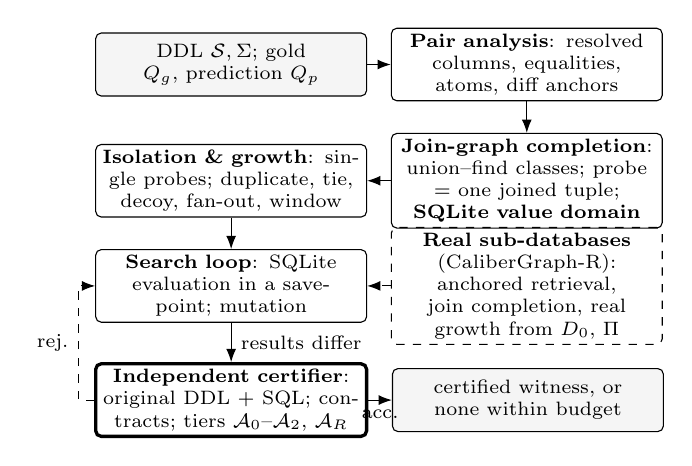
\begin{tikzpicture}[font=\scriptsize,>=Latex,
  box/.style={draw,rounded corners=2pt,align=center,inner sep=2pt,minimum height=8mm,text width=33mm},
  io/.style={box,fill=black!4},
  cert/.style={box,very thick}]
\node[io] (in) at (0,0) {DDL $\mathcal S,\Sigma$; gold $Q_g$, prediction $Q_p$};
\node[box,right=3mm of in] (an) {\textbf{Pair analysis}: resolved columns, equalities, atoms, diff anchors};
\node[box,below=4mm of an] (jg) {\textbf{Join-graph completion}: union--find classes; probe = one joined tuple; \textbf{SQLite value domain}};
\node[box,left=3mm of jg] (iso) {\textbf{Isolation \& growth}: single probes; duplicate, tie, decoy, fan-out, window};
\node[box,below=4mm of iso] (ev) {\textbf{Search loop}: SQLite evaluation in a savepoint; mutation};
\node[box,dashed,right=3mm of ev] (rs) {\textbf{Real sub-databases} (CaliberGraph-R): anchored retrieval, join completion, real growth from $D_0$, $\Pi$};
\node[cert,below=5mm of ev] (ce) {\textbf{Independent certifier}: original DDL + SQL; contracts; tiers $\mathcal A_0$--$\mathcal A_2$, $\mathcal A_R$};
\node[io,right=3mm of ce] (out) {certified witness, or none within budget};
\draw[->] (in)--(an);
\draw[->] (an)--(jg);
\draw[->] (jg)--(iso);
\draw[->] (iso)--(ev);
\draw[->,dashed] (rs)--(ev);
\draw[->] (ev)-- node[right,font=\scriptsize]{results differ} (ce);
\draw[->] (ce)-- node[below,font=\scriptsize]{acc.} (out);
\draw[->,dashed] (ce.west) -- ++(-2mm,0) |- node[pos=0.25,left,font=\scriptsize,align=right]{rej.} (ev.west);
\end{tikzpicture}
\caption{CaliberGraph pipeline. Candidates built from join-graph probes are evaluated by SQLite; a candidate that separates the queries is returned only if the independent certifier accepts it at the target tier. CaliberGraph-R (dashed) first searches real sub-databases of the benchmark database.}
\label{fig:overview}
\end{figure}


\textbf{Pair analysis and diff anchors.} Both queries are parsed in the SQLite dialect; column references are resolved to $(T,c)$ through aliases, subqueries and CTEs. For each query $Q$ we collect its tables $\mathrm{tab}(Q)$, its column equalities $E(Q)$ (including \texttt{IN}-subquery pairs) and its \emph{atoms} $\mathit{At}(Q)$: comparisons, \texttt{LIKE}, \texttt{IN}, \texttt{BETWEEN} and \texttt{IS [NOT] NULL} between a column, optionally wrapped in one function (\texttt{strftime}, \texttt{substr}, \texttt{lower}, \texttt{CAST}, $\pm k$, \dots), and literals. The \emph{anchor atoms} are those whose normal form (resolved names, canonical operator) occurs in only one query, and the \emph{anchor columns} add every column referenced, projected, ordered, grouped or aggregated in only one query. Anchors localise where the queries can disagree.

\textbf{Join-graph completion.} Let $\mathcal T^{*}$ be $\mathrm{tab}(Q_g)\cup\mathrm{tab}(Q_p)$ closed under foreign-key parents. Columns of $\mathcal T^{*}$ are partitioned into classes by the closure of $E(Q_g)\cup E(Q_p)$ and of the foreign keys, computed with union--find. A \emph{probe} assigns one value per class; its materialisation contains one row per referenced table, so that all equated columns agree, and a repair step adds parent rows for dangling foreign keys, fills \texttt{NOT NULL} columns and drops duplicate keys. Key classes receive distinct values in distinct probes.

\begin{proposition}[Reachability]
If a probe makes every atom of the outermost \texttt{WHERE} clause of $Q$ true, its rows form a joined tuple of $Q$ that satisfies the join conditions and filters of $Q$ in the repaired database.
\end{proposition}
\noindent Each equality of $E(Q)$ relates columns of one class, which take one value; repair only adds rows, fills \texttt{NULL}s in \texttt{NOT NULL} columns and drops later duplicates, so the probe's rows are unchanged. Random rows satisfy a join only by chance, which is why fuzzing draws keys from tiny domains; probes reach the output by construction whenever their filters hold.

\textbf{SQLite-aware value domain.} Each class receives a pool of values from the atoms on its columns: each literal $v$ and $v\pm1$, $v\pm0.5$ for numeric columns (integer division, \texttt{CAST}); case and padding variants of strings (\texttt{=} is case-sensitive, \texttt{LIKE} is not); pre-images under wrapping functions (e.g.\ \texttt{'2012-06-15 10:00:00'} for \texttt{strftime('\%Y',$c$)='2012'}); matching and non-matching \texttt{LIKE} instances; and values strictly between two comparable literals. Values are coerced to the declared type, and text of an unobserved shape is replaced by an observed sample.

\textbf{Isolation and controlled growth.} Aggregates, \texttt{DISTINCT}, \texttt{GROUP BY} and \texttt{ORDER BY}\dots\texttt{LIMIT} can \emph{mask} a difference. The search therefore starts from single-probe databases, in which one joined tuple determines the output, and grows them only with operators that target a masking mechanism (Table~\ref{tab:operators}).

\begin{table}[t]
\centering\footnotesize
\caption{Growth operators (each followed by repair).}\label{tab:operators}
\begin{tabularx}{\linewidth}{@{}l>{\raggedright\arraybackslash}X@{}}
\toprule
Operator & Construction: difference exposed\\
\midrule
duplicate & row copy with fresh keys: \texttt{DISTINCT}, \texttt{COUNT(DISTINCT)}\\
fan-out & $n$ child rows of a join: multiplicity, \texttt{HAVING COUNT}$>n$\\
tie probe & fresh copy tied on ordered columns, both insertion orders: \texttt{LIMIT} tie-breaking\\
window & $\ell{+}o{+}1$ tie probes: rows at \texttt{LIMIT}~$\ell$ \texttt{OFFSET}~$o$ borders\\
literal cover & one probe per equality literal: \texttt{CASE} branches, \texttt{IN} lists\\
decoy & a row that joins nothing: outer joins, anti-joins, \texttt{NOT IN}\\
violating & a probe failing the filters: empty inputs, \texttt{MAX} over no row\\
\bottomrule
\end{tabularx}
\end{table}

\begin{algorithm}[t]
\caption{CaliberGraph (CaliberGraph-R adds line 4)}\label{alg:main}
\footnotesize
\begin{algorithmic}[1]
\Require DDL $(\mathcal S,\Sigma)$, queries $Q_g,Q_p$, tier $\mathcal A$, budget $B$; for $\mathcal A_R$: $D_0$, $\Pi$
\Ensure witness $W\in\mathcal A$ with $\neg\mathcal C_{\mathrm{set}}(Q_g(W),Q_p(W))$, or $\bot$
\State analyse $Q_g,Q_p$: equalities $E$, atoms $\mathit{At}$, anchors
\State union--find column classes over $\mathcal T^{*}$; a value pool per class
\State $\mathit{Pool}\gets\emptyset$
\State \textbf{if} $\mathcal A=\mathcal A_R$: put real sub-databases (anchored retrieval, join completion, real growth) first in the stream
\For{each $D$ in the candidate stream \textbf{while} time $<B$}
  \State $(r_g,r_p)\gets$ run $Q_g,Q_p$ on $D$ in a savepoint
  \If{$\mathrm{set}(r_g)\neq\mathrm{set}(r_p)$ \textbf{and} \Call{Certify}{$D,\mathcal A$}}
    \State \Return $D$ \Comment{re-certified on a fresh connection}
  \EndIf
  \State add $D$ to $\mathit{Pool}$ with weight $=$ number of non-empty results among $r_g,r_p$
\EndFor
\State \Return $\bot$
\Statex \emph{Candidate stream, in order:} single probes for $Q_g$, $Q_p$ and both; two-probe combinations; growth operators (Table~\ref{tab:operators}); boundary and \texttt{NULL} variants of anchor classes; then mutations of parents drawn from $\mathit{Pool}$ by weight, each followed by repair
\end{algorithmic}
\end{algorithm}

\textbf{Search and certification.} The candidate stream (Algorithm~\ref{alg:main}) enumerates single-probe databases satisfying $Q_g$, $Q_p$ and both, then two-probe combinations, the growth structures and boundary and \texttt{NULL} variants of anchor classes, and finally runs a mutation loop until the budget expires (parents weighted by how many queries return rows; 70\,\% of value changes on anchor columns). Each candidate is evaluated in a savepoint of one in-memory SQLite connection (a few hundred microseconds). A candidate on which the results differ is returned only if the certifier accepts it at the target tier, and the certifier is re-run on a fresh connection before reporting. \emph{Soundness} is immediate: a returned $W$ is in $\mathcal A$ and separates the original strings on SQLite. The guarantee is one-sided and relative to the correctness of SQLite and the certifier. CaliberGraph+SC (``SC'': SpotIt+ constraints) additionally uses the constraints mined by SpotIt+ for value pools and acceptance, so that it has the same knowledge as SpotIt+; no other self-run tool uses them.

\subsection{Data-grounded search for $\mathcal A_R$}\label{sec:realsearch}
CaliberGraph-R changes where candidate rows come from. It reads $D_0$ (through an indexed read-only copy) and $\Pi$, and searches \emph{real sub-databases} before synthesis. A sub-database of $D_0$ that is closed under the inclusion dependencies of $\Pi$ satisfies the profile, except for rare rows that violate an approximate cross-key dependency.
\begin{itemize}
\item \emph{Diff-anchored retrieval.} The atoms of each query on table $T$ are translated back to SQL predicates $\varphi_g^T,\varphi_p^T$; rows with $\varphi_g^T\wedge\neg\varphi_p^T$ or $\varphi_p^T\wedge\neg\varphi_g^T$ are retrieved first (the filters disagree on them), then rows satisfying both, one, or neither.
\item \emph{Join completion.} Each seed row is completed along the join graph with real related rows, preferably of the same predicate mode, and closed under foreign keys, undeclared foreign keys and total participation.
\item \emph{Real growth.} Sub-databases are combined (a row only one query selects next to rows both select) and grown with real rows that tie on an \texttt{ORDER BY} column, the first $k{+}1$ rows of a \texttt{LIMIT}~$k$ window, real \texttt{NULL}s and real duplicates; they are shrunk by single-row deletions, and an entity can be cloned with the rows that reference it.
\item \emph{Constrained synthesis.} If no real sub-database separates the queries, the synthetic search continues from the evaluated sub-databases with pools filtered by $\Pi$, untouched columns filled from real template rows, and a repair step that also enforces $\Pi$.
\end{itemize}

\textbf{Example (development pair).} For BIRD question 1020 (``Which player has the highest overall rating?''), $Q_g$ orders \texttt{Player\_Attributes} by \texttt{overall\_rating DESC LIMIT 1}, whereas the Alpha-SQL prediction selects every row equal to the maximum rating. Both return one player on $D_0$. CaliberGraph-R retrieves a real attribute record (rating 84) with its player, then adds a \emph{real} record of another player with the same rating. On this four-row database, every row of which occurs in BIRD, $Q_g$ returns one player and $Q_p$ two; the witness is certified at $\mathcal A_R$ after 28 candidates and 0.22\,s. Whether the prediction or the gold query is right depends on how the question treats ties, which is what attribution judges.

\section{Experimental Setup}\label{sec:setup}

\textbf{Benchmark and systems.} We use the 1,534 questions of the BIRD development set (2024-06-27 revision)~\cite{li2023bird} over eleven SQLite databases with 3--13 tables. Predictions come from the ten systems whose BIRD outputs were released with SpotIt+~\cite{tremante2026spotitplus}: Alpha-SQL~\cite{li2025alphasql}, CHESS~\cite{talaei2024chess}, CSC-SQL-7B/32B~\cite{sheng2025cscsql}, two GenaSQL submissions~\cite{donder2025genasql}, GSR (an anonymous entry listed in~\cite{tremante2026spotitplus}), OmniSQL-32B~\cite{li2025omnisql}, RSL-SQL~\cite{cao2024rslsql} and SLM-SQL~\cite{sheng2025slmsql}, covering multi-agent pipelines, fine-tuned 7B--32B models and self-consistency. BIRD is the only Text-to-SQL benchmark for which verifier outputs on many systems have been released, which lets us compare all tool families on identical inputs, and its databases are large real instances (3.9\,M rows), which tier $\mathcal A_R$ needs. We recomputed the released EX labels on the official databases; they agree on 15,339 of 15,340 pairs (the exception depends on the current date). The held-out schemas are \texttt{formula\_1}, \texttt{superhero} and \texttt{toxicology}. Development has 349 questions and test 1,174, i.e.\ 11,740 test (system, question) pairs: \V{nExc} EX-correct (6,456 distinct predictions) and 3,745 EX-incorrect.

\textbf{Baselines.} They cover the main families of judging a prediction beyond EX, each with a strong public representative for SQLite and BIRD:
\begin{itemize}
\item \emph{Random fuzzing} in the style of test-suite accuracy~\cite{zhong2020testsuite}: 1--5 random rows per referenced table with values from both queries' literals, observed value samples, type-faithful values and \texttt{NULL}; keys from a three-value domain so that joins occur; foreign and primary keys repaired. It shares CaliberGraph's value coercion and certifier, but no join graph, anchors or isolation.
\item \emph{ParSEval}~\cite{chen2025parseval} (commit \texttt{88cfe245}, Z3 4.16.0), coverage-driven symbolic generation. ParSEval-L1 keeps its generator but accepts only certified databases, restarts with new seeds until the budget is spent, and receives the same observed format samples; its unmodified \texttt{disprove} routine is reported as ParSEval (official). ParSEval's solver exceeded the budget and was stopped on 732 of the 6,456 distinct pairs.
\item \emph{SpotIt}~\cite{klopfenstein2026spotit} and \emph{SpotIt+}~\cite{tremante2026spotitplus}, bounded verification without and with LLM-validated mined constraints (released outputs).
\end{itemize}
\emph{Excluded tools.} Provers such as SQLSolver~\cite{ding2023sqlsolver} and QED~\cite{wang2024qed} establish equivalence and return no counterexample database; VeriEQL~\cite{he2024verieql} is represented by SpotIt, which builds on it and reports BIRD results; XData~\cite{chandra2015xdata} and EvoSQL~\cite{castelein2018evosql} generate tests for one query or a mutant space rather than for a given pair. LLM judges~\cite{kim2025flex} produce no checkable evidence.

For the second freeze, \emph{random fuzzing-R} draws 1--5 real rows per referenced table from $D_0$ or template rows, re-draws referenced columns from literals, observed values and \texttt{NULL}, and closes the result under foreign keys and total participation with real rows; \emph{ParSEval-R} gives ParSEval a value provider that returns observed values first; because its solver still introduces unobserved values, it is a weak baseline at this tier, and we do not claim a fair comparison with symbolic generation at $\mathcal A_R$. Both receive the same read access to $D_0$, profile, repair and certifier-in-the-loop acceptance at $\mathcal A_R$ as CaliberGraph-R.

\textbf{Budgets and platform.} All self-run tools get 5\,s wall-clock per distinct pair on one core (two workers on a 2-core VM with 7\,GB of memory); a 10\,s budget is evaluated on a random subsample of \V{nSub} distinct pairs, which is also used for ablations. ParSEval-R certified none of 600 development pairs and was therefore run on this subsample only (decided before the second test run). CaliberGraph is implemented in Python 3.13 with SQLGlot and SQLite 3.45. Code, splits, raw outputs, witnesses, certifier reports, annotations and the pre-registrations are in the artifact repository.

\section{Results}\label{sec:results}

All numbers are computed on the test questions by scripts from the saved outputs; counts are over (system, question) pairs unless stated otherwise. Table~\ref{tab:overview} summarises every tool at every tier and Table~\ref{tab:hypotheses} the pre-registered hypotheses; analyses that were not pre-registered are marked \emph{post hoc}.

% ICDE overview table; all numbers are macros from numbers.tex (generated by src/make_numbers.py)
\begin{table*}[t]
\centering\footnotesize
\caption{Overview on the test pairs. \emph{Certified}: EX-correct pairs ($n=\V{nExc}$) with a witness that our certifier accepts at each tier (re-certified for SpotIt/SpotIt+); \emph{Claimed}: pairs the released results classify as non-equivalent. \emph{Recall}: share of known positives ($n=\V{nExi}$) with a witness. \emph{Attribution}: random sample of 100 witnesses per tool at the tier given in parentheses; \emph{Est.\ meaningful}: certified count $\times$ meaningful share (95\,\% CI). --: not applicable or not sampled.}\label{tab:overview}
\setlength{\tabcolsep}{4pt}
\begin{tabular}{@{}l r rrrrr rr rrl@{}}
\toprule
& & \multicolumn{5}{c}{Certified EX-correct pairs} & \multicolumn{2}{c}{Recall (\%)} & \multicolumn{3}{c}{Attribution of witnesses}\\
\cmidrule(lr){3-7}\cmidrule(lr){8-9}\cmidrule(l){10-12}
Tool & Claimed & $\mathcal A_0$ & $\mathcal A_{1f}$ & $\mathcal A_2$ & $\mathcal A_{Rq}$ & $\mathcal A_R$ & $\mathcal A_{1f}$ & $\mathcal A_R$ & Impl.\,\% (tier) & Mean.\,\% & Est.\ meaningful [CI]\\
\midrule
SpotIt & \V{nSIClaims} & \V{nSILzero} & \V{nSILonef} & \V{nSILtwo} & \V{nSIAtRq} & \V{nSIAtR} & \V{rSI}$^{*}$ & -- & \V{pSIImpl} ($\mathcal A_0$) & \V{pSIMeaningful} & \V{estSIMeaningful} \V{estSIMeaningfulCI}\\
SpotIt+ & \V{nSIPClaims} & \V{nSIPLzero} & \V{nSIPLonef} & \V{nSIPLtwo} & \V{nSIPAtRq} & \V{nSIPAtR} & -- & -- & \V{pSIPImpl} ($\mathcal A_0$) & \V{pSIPMeaningful} & \V{estSIPMeaningful} \V{estSIPMeaningfulCI}\\
ParSEval (official) & -- & \V{nPVOLzero} & \V{nPVOLonef} & \V{nPVOLtwo} & -- & -- & -- & -- & -- & -- & --\\
ParSEval-L1 & -- & \V{nPVLzero} & \V{nPVLonef} & \V{nPVLtwo} & \V{nPVAtRq} & \V{nPVAtR} & \V{rPVLonef} & -- & \V{pPVImpl} ($\mathcal A_{1f}$) & \V{pPVMeaningful} & \V{estPVMeaningful} \V{estPVMeaningfulCI}\\
Random fuzzing & -- & \V{nFZLzero} & \V{nFZLonef} & \V{nFZLtwo} & \V{nFZAtRq} & \V{nFZAtR} & \V{rFZLonef} & -- & \V{pFZImpl} ($\mathcal A_{1f}$) & \V{pFZMeaningful} & \V{estFZMeaningful} \V{estFZMeaningfulCI}\\
CaliberGraph & -- & \V{nCGLzero} & \V{nCGLonef} & \V{nCGLtwo} & \V{nCGAtRq} & \V{nCGAtR} & \V{rCGLonef} & -- & \V{pCGImpl} ($\mathcal A_{1f}$) & \V{pCGMeaningful} & \V{estCGMeaningful} \V{estCGMeaningfulCI}\\
CaliberGraph+SC & -- & \V{nCGSCLzero} & \V{nCGSCLonef} & \V{nCGSCLtwo} & \V{nCGSCAtRq} & \V{nCGSCAtR} & -- & -- & -- & -- & --\\
\midrule
Random fuzzing-R & -- & \V{nFZRAtLonef} & \V{nFZRAtLonef} & \V{nFZRAtLtwo} & \V{nFZRAtRq} & \V{nFZRAtR} & \V{rFZRAtLonef} & \V{rFZRAtR} & \V{pFZRImpl} ($\mathcal A_R$) & \V{pFZRMeaningful} & \V{estFZRMeaningful} \V{estFZRMeaningfulCI}\\
CaliberGraph-R & -- & \V{nCGRAtLonef} & \V{nCGRAtLonef} & \V{nCGRAtLtwo} & \V{nCGRAtRq} & \V{nCGRAtR} & \V{rCGRAtLonef} & \V{rCGRAtR} & \V{pCGRImpl} ($\mathcal A_R$) & \V{pCGRMeaningful} & \V{estCGRMeaningful} \V{estCGRMeaningfulCI}\\
\bottomrule
\multicolumn{12}{@{}p{\dimexpr\textwidth-2pt}@{}}{\scriptsize $^{*}$Share of known positives SpotIt claims non-equivalent (uncertified). ParSEval-R certified none of the \V{nSubR} subsample pairs (Section~\ref{sec:setup}) and is omitted. The second-stage tools search at $\mathcal A_R$ only; their $\mathcal A_0$--$\mathcal A_2$ entries re-evaluate the same witnesses ($\mathcal A_R\subseteq\mathcal A_{1f}\subseteq\mathcal A_0$).}\\
\end{tabular}
\end{table*}

% ICDE: pre-registered hypotheses and outcomes; numbers are macros from numbers.tex / numbers_icde.tex
\begin{table}[t]
\centering\scriptsize
\caption{Pre-registered hypotheses and outcomes on the test pairs. $\Delta$: difference in pairs (H6: estimated meaningful witnesses) with 95\,\% CI from a bootstrap over questions; $p$: exact McNemar (H1--H5), Holm-adjusted within H1--H3 and (post hoc) across the four H4 components; one-sided bootstrap over questions for H6--H7. Stage~3: one-sided tests, Holm-adjusted over its eight tests (C1 and C2 share a row; C2: \V{arcApct} vs.\ \V{arcANpct}\,\%, adjusted $p$ \V{holmCTwo}); R2 and R3 were pre-registered separately and are not adjusted; SP1--SP2 were pre-registered separately and are Holm-adjusted together; $\kappa_2$: Cohen's $\kappa$ on implausible vs.\ other.}\label{tab:hypotheses}
\setlength{\tabcolsep}{3pt}
\begin{tabular}{@{}l p{27mm} l l c@{}}
\toprule
& Comparison & $\Delta$ [95\,\% CI] & $p$ & Result\\
\midrule
H1 & CG at $\mathcal A_{1f}$ vs SpotIt claims & \V{hOneDiff} \V{hOneCI} & $<10^{-10}$ & yes\\
H2 & CG+SC at $\mathcal A_2$ vs SpotIt+ claims & \V{hTwoDiff} \V{hTwoCI} & $<10^{-10}$ & yes\\
H3 & recall: CG vs ParSEval-L1 / SpotIt & \V{rCGLonef} vs \V{rPVLonef} / \V{rSI}\,\% & $<10^{-10}$ & yes\\
H4 & each component's removal lowers the count & join graph only ($-$11) & 0.004 & no\\
H5 & CG-R vs fuzzing-R at $\mathcal A_R$ & \V{tCGRvsFZRRDiff} \V{tCGRvsFZRRCI} & $<10^{-10}$ & yes\\
   & CG-R vs ParSEval-R (subsample) & \V{ablRFull} vs \V{ablRPV} & $<10^{-10}$ & \\
H6 & est.\ meaningful, CG-R vs fuzzing-R & \V{hSixDiff} \V{hSixClusterCI} & \V{hSixClusterP} & weak\\
H7 & implausible share, CG-R vs CG & \V{pCGRImpl} vs \V{pCGImpl}\,\% & $<10^{-4}$ & yes\\
\midrule
\multicolumn{5}{@{}l}{\emph{Stage 3 (attribution validity and replication)}}\\
A1 & humans without $D_0$ agree with each other & $\kappa_2$ \V{hvKappaHHbin} & & no\\
A2--3 & \quad with AI; tier gap & $\kappa_2$ \V{hvKappaHAbinMin}--\V{hvKappaHAbinMax}; \V{hvImpConsOne}/\V{hvConsOne} vs \V{hvImpConsTwo}/\V{hvConsTwo} & \V{holmAThree} & no\\
R2 & humans with facts of $D_0$: tier gap & \V{hvTwoImpConsOne}/\V{hvTwoConsOne} vs \V{hvTwoImpConsTwo}/\V{hvTwoConsTwo} & \V{hvTwoP} & yes\\
   & \quad agree with each other / with AI & $\kappa_2$ \V{hvTwoKappaBin} / \V{hvTwoKappaAIbinMax} & & yes / no\\
B & second model vs AI; tier gap & $\kappa_2$ \V{cmKappaBin}; \V{cmImpOne} vs \V{cmImpTwo}\,\% & \V{holmBTwo} & yes\\
C & our issues vs Arcwise-Plat corrections & \V{arcGpct} vs \V{arcNpct}\,\% (gold) & \V{holmCOne} & no\\
S1 & Spider: CG-R vs fuzzing-R at $\mathcal A_R$ & \V{spRCG} vs \V{spRFZ} & \V{holmSOne} & no\\
S2 & Spider: implausible, CG-R vs CG & \V{spImpCGR} vs \V{spImpCG} of 60 & \V{holmSTwo} & no\\
S3 & Spider: est.\ meaningful, CG-R vs fuzzing-R & \V{spEstCGR} vs \V{spEstFZR} & \V{holmSThree} & rev.\\
E1 & 13 new BIRD systems: CG-R vs fuzzing-R & \V{mdDiff} [\V{mdLo}, \V{mdHi}] & \V{holmEOne} & yes\\
R3-1 & three humans agree (Fleiss) & $\kappa_2$ \V{hvThreeFleissBin} & & no\\
R3-2 & \quad majority vs AI & $\kappa_2$ \V{hvThreeKappaAIbin} & & no\\
R3-3 & \quad majority: tier gap & \V{hvThreeImpOne}/\V{hvThreeMajOne} vs \V{hvThreeImpTwo}/\V{hvThreeMajTwo} & \V{hvThreePThree} & yes\\
R3-4 & \quad pred.\ errors at $\mathcal A_R$, majority vs AI & \V{hvThreeErrHumTwo} vs \V{hvThreeErrAITwo} of \V{hvThreeMajTwo} & \V{hvThreePFour} & yes\\
SP1 & CG vs SpotIt re-run, $\mathcal A_{1f}$ & \V{srOneDiff} \V{srOneCI} & $<10^{-10}$ & yes\\
SP2 & \quad at $\mathcal A_0$ & \V{srTwoDiff} \V{srTwoCI} & $<10^{-10}$ & yes\\
\bottomrule
\end{tabular}
\end{table}


\subsection{RQ1: Certified witnesses at schema-derived tiers}\label{sec:main}
At the primary tier $\mathcal A_{1f}$, CaliberGraph certifies \V{nCGLonef} of the \V{nExc} EX-correct pairs (\V{pCGLonef}\,\%). SpotIt's released results claim \V{nSIClaims}; CaliberGraph certifies \V{hOneDiff} more (95\,\% CI \V{hOneCI}), although SpotIt's claims are counted without certification and its per-pair time reaches about 20 minutes at the 95th percentile against our five seconds (H1). Under identical budgets, acceptance tests and format knowledge, ParSEval-L1 certifies \V{nPVLonef} pairs and random fuzzing \V{nFZLonef}; only \V{vsPVBOnly} and \V{vsFZBOnly} of their pairs lack a CaliberGraph witness. CaliberGraph's lead is specific to these tiers: at $\mathcal A_2$, whose LLM-validated constraints none of the three tools uses, random fuzzing certifies more pairs (\V{nFZLtwo} vs \V{nCGLtwo}); given those constraints, CaliberGraph+SC certifies \V{nCGSCLtwo} pairs against \V{nSIPClaims} claimed by SpotIt+ (H2). With the official full-column format profiles (a pre-registered sensitivity check), CaliberGraph keeps \V{nCGOonef} pairs, ParSEval-L1 \V{nPVOonef}, fuzzing \V{nFZOonef}, and SpotIt, SpotIt+ and CaliberGraph+SC none.

Released verifier counterexamples lose many pairs on re-certification: of SpotIt's \V{nSIClaims} claims, \V{nSILzero} counterexamples still separate the original queries on SQLite and satisfy the DDL, and \V{nSILonef} are also format-faithful (SpotIt+: \V{nSIPLzero} and \V{nSIPLonef} of \V{nSIPClaims}). On development data, the loss at $\mathcal A_0$ was traced mainly to preprocessing (upper-cased literals, unmodelled \texttt{NOT NULL} and \texttt{UNIQUE} constraints) rather than to wrong verdicts; the further loss comes from implausible value formats. Multiset equality leaves every count unchanged, and the lenient $\mathcal C_{\mathrm{len}}$ keeps \V{nCGLonefLenient} of CaliberGraph's \V{nCGLonef} pairs.


\subsection{RQ2: What do the witnesses show? (post hoc)}\label{sec:attrresults}
% generated by src_s3/s3a_table.py
\begin{table}[t]
\centering\scriptsize
\caption{Human estimates next to the AI estimates (pre-registered reporting rule): verdicts on the same blind items, per round and stage (stage 1: schema-tier witnesses; stage 2: $\mathcal A_R$). Humans: items on which both annotators agree; Dis.: they disagree. Round 1 showed only the witness, round 2 also facts of $D_0$.}\label{tab:humanai}
\setlength{\tabcolsep}{3pt}
\begin{tabular}{@{}llrrrrrrr@{}}
\toprule
Round & Stage, judge & $n$ & Pred.\ err. & Both & Gold err. & Ambig. & Implaus. & Dis.\\
\midrule
1 & 1, AI & 30 & 0 & 0 & 8 & 8 & 14 & \\
 & 1, humans & 30 & 8 & 0 & 18 & 1 & 0 & 3\\
\addlinespace[1pt]
 & 2, AI & 30 & 4 & 0 & 7 & 12 & 7 & \\
 & 2, humans & 30 & 11 & 1 & 11 & 1 & 0 & 6\\
\midrule
2 & 1, AI & 30 & 3 & 1 & 4 & 6 & 16 & \\
 & 1, humans & 30 & 4 & 0 & 1 & 0 & 20 & 5\\
\addlinespace[1pt]
 & 2, AI & 30 & 3 & 1 & 3 & 12 & 11 & \\
 & 2, humans & 30 & 14 & 0 & 2 & 1 & 9 & 4\\
\bottomrule
\end{tabular}
\end{table}



\begin{figure}[t]
\centering
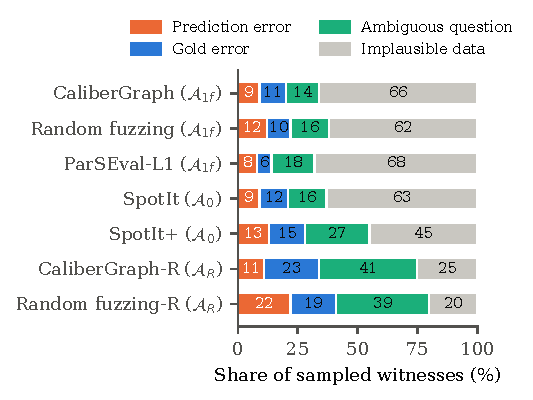
\includegraphics[width=\linewidth]{figs/attribution.pdf}
\caption{Attribution of random samples of 100 witnesses per tool (LLM annotation: two tool-blind passes, adjudicated). Upper five bars: first-stage tools at $\mathcal A_{1f}$ (SpotIt and SpotIt+ at $\mathcal A_0$); lower two: second-stage tools at $\mathcal A_R$.}\label{fig:attribution}
\end{figure}

The two annotation passes agree on \V{attrAgree}\,\% of the \V{attrN} first-stage witnesses ($\kappa=\V{attrKappa}$); \V{attrAdj} disagreements were adjudicated. For every tool, \V{attrImplMin}--\V{attrImplMax}\,\% of the sampled witnesses separate the queries only on implausible data, and only \V{attrErrMin}--\V{attrErrMax}\,\% expose an error of the prediction (Fig.~\ref{fig:attribution}; CaliberGraph: \V{pCGImpl}\,\% implausible, CI over questions \V{pCGImplClusterCI}). The decisive implausible facts are of few kinds: \texttt{NULL} in a column that is never \texttt{NULL} in BIRD; duplicates of what is unique in reality (a badge awarded twice, two races of one Grand Prix in a season); values that do not occur (a negative round, an atom identifier of the wrong pattern); and inconsistent records (a school whose county differs between two tables, a bond stored in one direction, an account without owner). Weighted by certified counts, CaliberGraph yields an estimated \V{estCGMeaningful} meaningful witnesses \V{estCGMeaningfulCI} and random fuzzing \V{estFZMeaningful} \V{estFZMeaningfulCI}: CaliberGraph's lead of \V{vsFZDiff} certified pairs over fuzzing does \emph{not} carry over to meaningful witnesses, and the estimated prediction errors its witnesses expose (\V{estCGErr}) are not more than fuzzing's (\V{estFZErr}). Of the \V{nSIClaims} pairs SpotIt claims to be non-equivalent, \V{nSILzero} can be re-certified, and an estimated \V{estSIErr} of these expose a prediction error. Since attribution judges the returned witness, not the pair, these are lower bounds on errors among certified pairs.

\textbf{Is the attribution valid? (Stage 3, pre-registered.)} Two human annotators labelled random samples of witnesses, half from each stage, independently and blind to tool, tier and AI verdict, in two rounds of \V{hvN} new witnesses each. In round~1 they saw only the witness and the queries: they agreed with each other on \V{hvAgreeHH} labels ($\kappa=\V{hvKappaHH}$; on implausible vs.\ other, $\kappa_2=\V{hvKappaHHbin}$) but not with the AI ($\kappa=\V{hvKappaHAmin}$--\V{hvKappaHAmax}), and each chose \emph{implausible data} only \V{hvHImpOne} times in 60 items, on different items, and \V{hvImpHOne} and \V{hvImpHTwo} times among the 30 first-stage witnesses, where the AI chose it \V{hvImpAIOne} times. Many of their reasons describe the anomaly the AI cites --- e.g., a lookup row \texttt{(3,'Bad')} where BIRD stores \texttt{(3,'Neutral')} --- but resolve it as an error of one query \emph{on the witness}. In round~2 every item also showed mechanically generated facts about $D_0$ (\texttt{NULL} counts, uniqueness and frequencies of the witness values of every referenced column), and the instructions asked first whether the difference could arise on real data. The annotators now chose \emph{implausible data} \V{hvTwoImpHOne} times each, agreed on it ($\kappa_2=\V{hvTwoKappaBin}$, CI \V{hvTwoKappaBinLo}--\V{hvTwoKappaBinHi}), and reproduced the difference between the tiers (\V{hvTwoImpConsOne} of the \V{hvTwoConsOne} first-stage and \V{hvTwoImpConsTwo} of the \V{hvTwoConsTwo} second-stage witnesses on which both agreed; one-sided Fisher $p=\V{hvTwoP}$), but agreed with the AI item by item only moderately ($\kappa_2=\V{hvTwoKappaAIbinMax}$, below the pre-registered 0.60). The shares we report in Fig.~\ref{fig:attribution} and below are the AI's and carry this uncertainty. ($\kappa_2$: Cohen's $\kappa$ on implausible vs.\ other.) Beyond implausibility, humans and AI also differ in the other labels (Table~\ref{tab:humanai}; five-label $\kappa$ \V{hvTwoKappaHAfiveMin}--\V{hvTwoKappaHAfiveMax} in round~2): the humans call many more witnesses prediction errors and almost none ambiguous, so every share of meaningful labels we report from the AI attribution should be read next to this table. A second model (Claude Sonnet~5.5) with the AI annotator's prompt and data access agreed with it on \V{cmN} witnesses ($\kappa=\V{cmKappaBin}$) and reproduced the drop between the stages (\V{cmImpOne} vs.\ \V{cmImpTwo} of 100).

\textbf{An annotator-free test (post hoc).} We repaired each first-stage witness locally, replacing the cells that violate the data profile $\Pi$ (Section~\ref{sec:profile}) by real values in 20 random repairs, and re-ran both queries. The difference vanished on every repair for \V{xVan} of \V{xN} witnesses (\V{xVanPct}\,\%) and survived on some for \V{xSurv}; it vanished for \V{xImpVanPct}\,\% of the witnesses the AI called implausible, but also for \V{xOthVanPct}\,\% of the others, and it vanished for \V{xHumVan} of the \V{xHumRep} repaired first-stage witnesses that both round-2 annotators called implausible. Yet for \V{xVanPairARpct}\,\% of the witnesses whose difference vanished (and \V{xPairARpct}\,\% of all), CaliberGraph-R or fuzzing-R found an $\mathcal A_R$ witness for the same pair: the two queries do differ on realistic data, but the first-stage witness does not show it. Without the facts, the round-1 annotators judged the \emph{pair} (which query answers the question); the AI, the round-2 annotators and the repair test judge the \emph{witness} (whether this database is evidence of that difference). The three are not independent of our definition: the facts shown in round~2 and the cells the repair replaces both come from $D_0$ and its profile, so they test the consistency of an operational notion of realism, not realism itself.


\subsection{RQ3: Data-grounded witnesses}\label{sec:rresults}

\begin{table}[t]
\centering\footnotesize
\caption{The data profile $\Pi$ mined from the eleven BIRD databases (75 tables, 3.9\,M rows; 258\,s on one core) and the share of first-stage $\mathcal A_{1f}$ witnesses (distinct EX-correct pairs) that violate each constraint class on the columns either query references (post hoc). CG: CaliberGraph; PSE: ParSEval-L1.}\label{tab:profile}
\setlength{\tabcolsep}{2pt}\scriptsize
\Tab{profile_icde}
\end{table}

None of CaliberGraph's \V{nCGLonef} first-stage witnesses satisfies the full data profile, and \V{nCGAtRq} satisfy it on the referenced columns. Column-level mined constraints do not close the gap: CaliberGraph+SC certifies \V{nCGSCLtwo} pairs at $\mathcal A_2$ but only \V{nCGSCAtR} at $\mathcal A_R$, none of SpotIt+'s \V{nSIPLtwo} $\mathcal A_2$ counterexamples reaches $\mathcal A_R$, and \V{pSIPImpl}\,\% of SpotIt+'s sampled witnesses are implausible. CaliberGraph-R certifies \V{nCGRAtR} EX-correct pairs (\V{pCGRAtR}\,\%) at $\mathcal A_R$, against \V{nFZRAtR} for random fuzzing-R with the same data access, repair and acceptance (difference \V{tCGRvsFZRRDiff}, CI \V{tCGRvsFZRRCI}); ParSEval-R certifies \V{ablRPV} of the \V{nSubR} subsample pairs, on which CaliberGraph-R certifies \V{ablRFull}. H5 is supported, and the lead holds on the schemas held out in the first stage, which informed the tier's design (\V{rateCGRHeld} vs \V{rateFZRHeld}\,\% of EX-correct pairs), as on the others (\V{rateCGROther} vs \V{rateFZROther}\,\%).

\textbf{Why schema-tier witnesses fail the profile (post hoc).} On the columns the queries reference (Table~\ref{tab:profile}), 72--86\,\% of the first-stage witnesses use a value outside the column's observed domain (an unseen category, shape or range), 30--70\,\% put a \texttt{NULL} into one of the 420 columns that are never \texttt{NULL} in BIRD, and 20--56\,\% break a value dependency (e.g., a county code paired with another county's name); half of ParSEval's minimal instances also duplicate a unique column combination. Every constraint class is violated by some tool's witnesses. Certified counts are insensitive to the categorical thresholds of the profile: re-certifying the stored witnesses with halved or doubled thresholds changes CaliberGraph-R's distinct certified pairs from \V{thrCGRFrozen} to \V{thrCGRLooser} or \V{thrCGRStricter}, fuzzing-R's from \V{thrFZRFrozen} to \V{thrFZRLooser} or \V{thrFZRStricter}, and admits none of CaliberGraph's first-stage witnesses.

\textbf{What the tier changes.} \V{pCGRImpl}\,\% of CaliberGraph-R's sampled witnesses rely on implausible data (CI over questions \V{pCGRImplClusterCI}), against \V{pCGImpl}\,\% of CaliberGraph's $\mathcal A_{1f}$ witnesses (H7; one-sided $p=\V{hSevenP}$, and $p\V{hSevenClusterP}$ over questions; pass agreement \V{attrRAgree}\,\%, $\kappa=\V{attrRKappa}$). The drop holds on the first-stage held-out schemas (\V{implCGRHeld} vs \V{implCGHeld}) and on the others (\V{implCGROther} vs \V{implCGOther}); fifty first-stage witnesses re-annotated in the same batch received the same verdict in \V{calibSame} cases, so it is not annotator drift. The rise in the meaningful share is due to the tier, not to the search: random fuzzing-R reaches \V{pFZRMeaningful}\,\%. CaliberGraph-R yields an estimated \V{estCGRMeaningful} meaningful witnesses against \V{estFZRMeaningful} for fuzzing-R; the difference (\V{hSixDiff}) was significant under the pre-registered parametric bootstrap (CI \V{hSixCI}, $p=\V{hSixP}$) but not robustly so under a bootstrap over questions (CI \V{hSixClusterCI}, one-sided $p=\V{hSixClusterP}$), so we regard H6 as only weakly supported. Post hoc, fuzzing-R's witnesses show a prediction error more often (estimated \V{estFZRErr} against \V{estCGRErr}); as its certified pairs are almost a subset of CaliberGraph-R's (\V{tCGRvsFZRRBOnly} exceptions), the difference lies in \emph{which} witness is returned for a pair.

\textbf{A limitation of the tier.} A sub-database may omit the entity a question names, so that one query returns no row and the other a row of \texttt{NULL}s; \V{nEmptyNullCGR} of CaliberGraph-R's and \V{nEmptyNullFZR} of fuzzing-R's 100 sampled witnesses are of this kind. Under $\mathcal C_{\mathrm{len}}$, which equates the two, CaliberGraph-R certifies \V{nCGRAtRClen} pairs and fuzzing-R \V{nFZRAtRClen}.

\textbf{A meaningful data-grounded witness.} For ``How many cards available in paper have a positive starting maximum hand size?'' the evidence defines availability as \texttt{LIKE '\%paper\%'}, but the gold query tests \texttt{availability = 'paper'}; CaliberGraph-R returns three real cards, one with the observed value \texttt{'arena,mtgo,paper'}, on which the gold query counts one card and the prediction two --- a gold query that contradicts its own evidence.

\textbf{Recall on known positives.} CaliberGraph finds an $\mathcal A_{1f}$ witness for \V{rCGLonef}\,\% of the \V{nExi} known positives, against \V{rPVLonef}\,\% for ParSEval-L1, \V{rFZLonef}\,\% for fuzzing and \V{rSI}\,\% claimed by SpotIt (H3). At $\mathcal A_R$ the figure is a sanity check rather than an estimate: $D_0$ itself separates every known positive and satisfies its profile up to the approximate cross-key rules, and CaliberGraph-R finds a witness for \V{rCGRAtR}\,\% (fuzzing-R \V{rFZRAtR}\,\%). No recall estimate exists for EX-correct pairs, on which a missed difference is invisible.


\subsection{RQ4: Effect on accuracy and rankings}\label{sec:rankings}

\begin{table}[t]
\centering\footnotesize
\caption{Per-system effect on the 1,174 test questions. Count-based: share of EX-correct predictions with a CaliberGraph $\mathcal A_{1f}$ witness, and EX after removing all of them (EX$'$). Error-weighted: certified share $\times$ attributed prediction-error rate (\V{errShareCG}\,\% at $\mathcal A_{1f}$, \V{errShareCGR}\,\% at $\mathcal A_R$), in points of EX; a lower bound (post hoc).}\label{tab:systems}
\setlength{\tabcolsep}{3pt}
\Tab{systems_icde}
\end{table}

Counting every $\mathcal A_{1f}$ witness as an error, \V{fpShareMin}--\V{fpShareMax}\,\% of each system's EX-correct predictions are removed, EX drops by \V{exDropMin}--\V{exDropMax} points and six to eight of the ten systems change rank, depending on how two exact EX ties are broken (Kendall's $\tau_b=\V{kendallTau}$; Table~\ref{tab:systems}); SpotIt's claims imply \V{ptsCountSpotItMin}--\V{ptsCountSpotItMax} points. RQ2 shows that most of these witnesses are not errors. Weighting each tool's certified share by its attributed prediction-error rate gives \V{ptsErrOnefMin}--\V{ptsErrOnefMax} points per system at $\mathcal A_{1f}$ and \V{ptsErrRMin}--\V{ptsErrRMax} at $\mathcal A_R$ (post hoc), with rankings unchanged except within the two exact ties ($\tau_b=\V{tauErrOnef}$ at both tiers); since one error rate is applied per tier, the rankings follow the certified shares, which differ little between systems. The estimates are lower bounds, since a pair whose returned witness is implausible may still be an error, and the error rate of each sample is uncertain (CaliberGraph-R: \V{errShareCGR}\,\%, interval over questions about 5--18\,\%). They also depend on who attributes: with the human annotators' pooled error rates (post hoc; \V{humErrPctOnef}\,\% of agreed schema-tier and \V{humErrPctR}\,\% of agreed $\mathcal A_R$ witnesses, Table~\ref{tab:humanai}), the same weighting gives \V{ptsHumOnefMin}--\V{ptsHumOnefMax} points at $\mathcal A_{1f}$ and \V{ptsHumRMin}--\V{ptsHumRMax} at $\mathcal A_R$, where counting every witness gives \V{ptsCountRMin}--\V{ptsCountRMax}. Data grounding thus changes what witnesses mean much more than how many errors they expose: the estimated prediction errors are similar at both tiers (\V{estCGErr} and \V{estCGRErr} for CaliberGraph and CaliberGraph-R). By the AI attribution, 58--64\,\% of the sampled $\mathcal A_R$ witnesses point to gold-query defects or ambiguities, some on sub-databases without the entity the question names; the human annotators disagree, attributing about half of the agreed $\mathcal A_R$ witnesses to prediction errors and almost none to ambiguity.


\subsection{RQ5: Ablation, cost and benchmark issues}\label{sec:ablation}

\begin{table}[t]
\centering\footnotesize
\caption{Ablation on a random subsample of \V{nSub} distinct EX-correct test pairs (5\,s per pair). Left: first stage, $\mathcal A_{1f}$ (H4). Right: second stage, $\mathcal A_R$, with baselines on the same subsample.}\label{tab:ablation}
\setlength{\tabcolsep}{3pt}
\begin{tabular}{@{}lrr@{}}
\toprule
Configuration & $\mathcal A_{1f}$ & $\Delta$\\
\midrule
CaliberGraph & \V{subFull} & \\
$-$anchoring & \V{subNoAnchor} & +1\\
$-$isolation & \V{subNoIso} & +2\\
$-$join graph & \V{subNoJoin} & $-$11\\
$-$SQLite domain & \V{subNoDomain} & +2\\
budget 10\,s & \V{subTen} & 0\\
ParSEval-L1 5\,s/10\,s & \multicolumn{2}{r}{\V{subPVFive}/\V{subPVTen}}\\
\bottomrule
\end{tabular}\hfill
\begin{tabular}{@{}lrr@{}}
\toprule
Configuration & $\mathcal A_R$ & $\Delta$\\
\midrule
CaliberGraph-R & \V{ablRFull} & \\
$-$real sub-DBs & \V{ablRNoReal} & $-$48\\
$-$synthesis & \V{ablRNoSyn} & $-$5\\
$-$anchoring & \V{ablRNoAnchor} & $-$11\\
$-$join completion & \V{ablRNoJoin} & $-$8\\
Random fuzzing-R & \V{ablRFuzz} & \\
ParSEval-R & \V{ablRPV} & \\
\bottomrule
\end{tabular}
\end{table}

\begin{figure}[t]
\centering
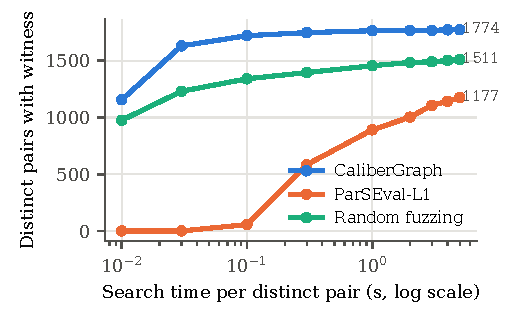
\includegraphics[width=0.92\linewidth]{figs/time_to_witness.pdf}
\caption{Distinct EX-correct pairs with a certified $\mathcal A_{1f}$ witness found within a given search time (first stage, 5\,s budget; a solver run that overruns the budget is not counted, so ParSEval-L1 reaches 1,177 of its 1,196 pairs).}\label{fig:time}
\end{figure}

In the first stage, join-graph completion is the only component whose removal lowers the count significantly (\V{hFourNoJoinFullOnly} of \V{subFull} pairs lost, none gained; Holm-adjusted $p=0.004$); removing anchoring, isolation or the SQLite value domain changes the count by at most two pairs, and the median time to a witness stays at 6--8\,ms. \textbf{H4 is not supported}: the differences these components target are also reached by the other phases and by the mutation loop, which applies the same operators at random, so their benefit on development pairs did not carry over. In the second stage, the real sub-database phase accounts for most witnesses (\V{ablRNoReal} without it, $p=\V{ablRNoRealP}$, fewer than fuzzing-R), and anchored retrieval ($p=\V{ablRNoAnchorP}$) and join completion ($p=\V{ablRNoJoinP}$) also contribute, whereas constrained synthesis adds few witnesses ($p=\V{ablRNoSynP}$).

\textbf{Cost.} When CaliberGraph finds an $\mathcal A_{1f}$ witness, the median search time is \V{tCGMedian}\,s (\V{tCGWithinOne}\,\% within 1\,s; Fig.~\ref{fig:time}); ParSEval-L1 needs \V{tPVMedian}\,s and CaliberGraph-R \V{tCGRRMedian}\,s at $\mathcal A_R$, including its queries to $D_0$. Most distinct pairs, however, end without a witness after the full budget, so the budget dominates the cost: auditing the accepted test predictions of one system (about 800) alone with CaliberGraph-R takes \V{costSysMean} core-hours on average (\V{costSysMin}--\V{costSysMax}), or 6.9 core-hours for all ten systems when identical predictions are shared. Doubling the budget leaves CaliberGraph's count unchanged and raises ParSEval-L1's from \V{subPVFive} to \V{subPVTen}; at $\mathcal A_R$ (post hoc, same subsample) it changes CaliberGraph-R's count from 195 to 193 and fuzzing-R's from 151 to 153, so neither stage is budget-bound. Mining the profile is a one-time cost per benchmark (Section~\ref{sec:profile}). Attribution, which F2 (Table~\ref{tab:findings}) makes necessary, is a manual or model-assisted cost of a sample per tool and is not included.

\textbf{Root causes and benchmark issues.} In a sample of 100 first-stage CaliberGraph witnesses, AI-annotated in two passes, \texttt{NULL} handling (30\,\%), filter predicates (18\,\%) and join paths (17\,\%) cause two thirds of the differences, followed by ordering and \texttt{LIMIT} ties (12\,\%), duplicates (9\,\%) and aggregates over empty input (8\,\%). Across all attribution samples (77 items from schema-tier samples, 46 from $\mathcal A_R$ samples), \V{nIssues} distinct test questions received a witness that the AI annotators judged to expose a gold-query defect (\V{nIssuesGold}) or an ambiguous question (\V{nIssuesAmb}). \V{nIssuesFragile} of them are fragile: their witness lacks the entity the question names, or the two results differ only in rounding or letter case; the remaining \V{nIssuesRobust} comprise \V{nIssuesRobustGold} gold defects and \V{nIssuesRobustAmb} ambiguities. The gold defects are \emph{latent}: on $D_0$ the gold query returns the accepted answer, but on the witness it answers the question wrongly. Recurrent kinds are wrong join paths or attributes (11), filters that contradict the question's evidence (8: inclusive \texttt{BETWEEN} for strict bounds, equality for \texttt{LIKE}, case-sensitive matches), aggregates over an empty selection that return \texttt{NULL} where a count of zero is meant (7), counts of rows or names where entities are counted (7), and averages that count \texttt{NULL}s (3); about half of the ambiguities concern ties. We release the list, with one witness, the annotators' reasons and these flags per question, as a candidate list for maintainers rather than a verdict. The list overlaps only weakly with the corrected annotations of Jin et al.~\cite{jin2026annotation} (pre-registered): of the \V{arcG} questions we flag as gold defects that their Arcwise-Plat set covers, \V{arcGk} (\V{arcGpct}\,\%) received a gold query with a different result on $D_0$, against \V{arcNpct}\,\% of the \V{arcNN} unflagged test questions (one-sided Fisher $p=\V{arcPone}$); our ambiguity flags do not predict their edits (\V{arcApct}\,\% vs.\ \V{arcANpct}\,\%). Counting textual corrections of the gold query, which our witnesses can expose although the corrected query returns the same result on $D_0$, the rate is \V{arcGtextPct}\,\% against \V{arcNtextPct}\,\% (post hoc). \V{arcGuntouched} flagged gold defects and \V{arcAuntouched} flagged ambiguities were left entirely unchanged by Arcwise-Plat.


\subsection{RQ6: Replication on Spider and on new systems (Stage 3)}\label{sec:replication}
We re-ran the frozen code on Spider~1.0 dev~\cite{yu2018spider}, which no design decision had seen: 20 databases (\V{spTables} tables, \V{spRows}\,k rows), 1,034 questions and six public prediction sets (DAIL-SQL~\cite{gao2024dailsql} with and without self-consistency, Graphix-T5~\cite{li2023graphix}, DIN-SQL~\cite{pourreza2023dinsql}, GPT-4 few- and zero-shot), i.e., \V{spN} EX-correct pairs. The pattern of the tiers replicates: CaliberGraph certifies \V{spCG} pairs at $\mathcal A_{1f}$ but \V{spCGR} at $\mathcal A_R$, fuzzing \V{spFZ} and \V{spFZR}. The search does not: CaliberGraph-R and fuzzing-R certify \V{spRCG} and \V{spRFZ} pairs at $\mathcal A_R$ (\V{spSOneA} vs.\ \V{spSOneB} discordant; one-sided $p=\V{spSOneP}$, CI over questions \V{spSOneLo} to \V{spSOneHi}; pre-registered S1 not supported), with equal recall on known positives (\V{spRecCGR} vs.\ \V{spRecFZR}\,\%). The attribution (two passes, $\kappa=\V{spKappa}$) finds \V{spImpCG} of \V{spNCG} sampled CaliberGraph witnesses implausible at $\mathcal A_{1f}$ against \V{spImpCGR} of \V{spNCGR} CaliberGraph-R witnesses at $\mathcal A_R$ (one-sided Fisher $p=\V{spSTwoP}$, not significant after Holm correction over the Stage-3 family) and none of \V{spNFZR} fuzzing-R witnesses; the estimated meaningful $\mathcal A_R$ witnesses are \V{spEstCGR} for CaliberGraph-R and \V{spEstFZR} for fuzzing-R (pre-registered S3 reversed: the difference has CI \V{spSThreeLo} to \V{spSThreeHi}, in fuzzing-R's favour). Post hoc, the implausible CaliberGraph-R witnesses almost all duplicate a real entity under a fresh key (two identical teachers), which the Spider profile does not forbid: on small tables our miner keeps only \V{spUcc} unique column combinations (BIRD: \V{bdUcc}), and \V{spCatShare}\,\% of the columns are categorical (BIRD: \V{bdCatShare}\,\%), so every admissible witness is close to a real sub-database and random real rows suffice.

On BIRD, the result of the search does replicate on systems the study had not seen: for the thirteen public prediction sets of BIRD Mini-Dev (GPT-3.5/4/4o, Llama-3, Mixtral, Phi-3), restricted to held-out test questions and to (question, prediction) pairs not seen before, CaliberGraph-R certifies \V{mdCGR} of \V{mdN} new EX-correct pairs at $\mathcal A_R$ and fuzzing-R \V{mdFZR} (\V{mdA} vs.\ \V{mdB} discordant; CI over questions \V{mdLo}--\V{mdHi}; Holm-adjusted $p$ \V{holmEOne}). Of \V{mdAttrN} sampled CaliberGraph-R witnesses, \V{mdImp} were attributed to implausible data, close to the second-stage share (\V{pCGRImpl}\,\%), and \V{mdErr} to a prediction error.


\section{Lessons and Threats to Validity}\label{sec:threats}

% ICDE: summary of findings and recommendations
\begin{table*}[t]
\centering\footnotesize
\caption{Summary of findings and recommendations.}\label{tab:findings}
\begin{tabularx}{\textwidth}{@{}l >{\raggedright\arraybackslash}X >{\raggedright\arraybackslash}X l@{}}
\toprule
& Finding (evidence) & Recommendation & Audience\\
\midrule
F1 & Under one SQLite certifier, released counterexamples lose about half of their pairs at the DDL tier and 82--92\,\% at the format tier; the ranking of tools changes with the tier (Sec.~\ref{sec:main}). & Compare disprovers only under one certifier, tier and budget; re-certify released witnesses on the benchmark's engine. & tool authors\\
F2 & By an LLM attribution, \V{attrImplMin}--\V{attrImplMax}\,\% of every tool's schema-tier witnesses rely on implausible data; humans shown facts of the data reach a similar verdict (\V{hvTwoImpConsOne}/\V{hvTwoConsOne} agreed items) but agree with the AI only moderately per item; humans without the facts almost never do; a repair test removes \V{xVanPct}\,\% of the differences (Sec.~\ref{sec:attrresults}). & Report witnesses with an attributed sample and the data facts the judgement rests on, never bare ``non-equivalent'' counts. & tool authors, maintainers\\
F3 & A data profile of the benchmark (minutes to mine) cuts implausible witnesses from \V{pCGImpl}\,\% to \V{pCGRImpl}\,\%; SpotIt+'s counterexamples (LLM-validated column constraints) are \V{pSIPImpl}\,\% implausible; re-certified counts are insensitive to the profile's thresholds (Sec.~\ref{sec:rresults}). & Publish the data profile with the benchmark; judge witnesses at $\mathcal A_R$, with a presupposition constraint for entities named in the question. & maintainers\\
F4 & The effect of witnesses on EX lies between \V{ptsErrRMin}--\V{ptsErrOnefMax} points per system (weighted by attributed error rates; a lower bound) and 15--20 points (all schema-tier witnesses counted) (Sec.~\ref{sec:rankings}). & Never subtract witness counts from EX; use meaningful witnesses to repair gold queries and questions. & maintainers, system builders\\
F5 & Join-graph completion and real-row retrieval matter; three synthetic components do not; a data-grounded audit of one system's accepted test predictions costs under one core-hour at 5\,s per pair, plus attribution (Sec.~\ref{sec:ablation}). & Build disprovers on the join graph and real data; certify and attribute every leaderboard submission. & tool authors, maintainers\\
F6 & On Spider, schema-tier witnesses again fail the profile, but CaliberGraph-R's lead does not replicate and fuzzing-R's witnesses are more meaningful; on 13 unseen BIRD systems the lead in counts replicates (Sec.~\ref{sec:replication}). & Mine profiles from instances large enough to expose keys and dependencies, or add them by hand. & maintainers, tool authors\\
\bottomrule
\end{tabularx}
\end{table*}

\textbf{Lessons.} Table~\ref{tab:findings} maps each finding to a recommendation. The common thread is that a counterexample is a database and should be judged as data: certified on the benchmark's engine with the original query strings, checked against the benchmark's own profile, and released so that others can attribute it. Meaningful witnesses are as much feedback on the benchmark as on the systems: 58--64\,\% of the sampled data-grounded witnesses expose latent gold-query defects or ambiguous questions (some on sub-databases without the named entity), against 11--22\,\% that expose prediction errors, and no correction of system scores can fix the former.

\textbf{Disproving is not proving.} A missing witness says nothing; accuracy corrected with witnesses is an upper bound on semantic accuracy, and error-weighted corrections are lower bounds on the over-statement. Bounded verifiers can also report the absence of counterexamples up to a bound, which our tools cannot.

\textbf{What ``implausible'' means.} The profile is mined from one instance, so it can be too strict (a plausible but unobserved value is admitted only through range and shape rules) and too weak: annotators still found conditional constraints it does not express (a badge awarded once while others repeat), which conditional-dependency and denial-constraint discovery could capture~\cite{fan2011cfd,chu2013dc}. ``Implausible'' combines absence from the instance with the annotators' judgement about the domain; a live football database may well contain unplayed fixtures without scores (Fig.~\ref{fig:example}). Sub-databases can also omit the entity a question names (Section~\ref{sec:rresults}). Some differences rely on behaviour SQL leaves unspecified, such as which tied row \texttt{LIMIT} keeps; BIRD's EX is computed with SQLite, so we count them, and attribution classifies most as ambiguities.

\textbf{AI-performed annotation.} All attribution and root-cause labels were produced by the AI model that also implemented the tools, in two independent passes plus adjudication; agreement between passes measures consistency, not correctness. A second model reproduces the labels (Section~\ref{sec:attrresults}), but both share a vendor and the same data access. The first author's earlier checks of two samples of 30 witnesses (agreement 26--28 of 30) were not blind: the AI verdicts were printed on the same sheet. The two human annotators, data analysts familiar with SQL who volunteered, labelled independently. The pre-registered blind check failed in its first round, in which they had no access to $D_0$; in a second, separately pre-registered round with facts from $D_0$ they agreed with each other and reproduced the difference between the tiers, but agreed with the AI only moderately item by item, so the AI's estimated shares carry this uncertainty. The two round-2 sheets returned to us contained a few manual edits outside the label fields (end-of-file markers, two altered witness cells in one item and a shortened fact line in another, both labelled alike by the two annotators; excluding the two items changes no outcome); the authors confirm that both rounds were annotated by hand without AI tools, and the sheets are released as received. Blinding to the tier is imperfect, since synthetic values (\texttt{'x1'}, \texttt{-1}) are recognisable. All annotations, reasons, witnesses and both human sheets are released.

\textbf{Baselines.} SpotIt and SpotIt+ are used through their released outputs because their constraint mining needs an LLM API unavailable in our environment; their budgets are larger than ours. ParSEval-R certifies nothing at $\mathcal A_R$ and is not a fair representative of symbolic generation there. The frozen first-stage fuzzing baseline accepted the first differing database without consulting the certifier, unlike every other tool; we re-ran exactly the affected pairs (132 distinct EX-correct, 259 EX-incorrect) with certifier-in-the-loop acceptance and the same seeds and report the corrected counts; its attribution sample was drawn before the correction.

\textbf{Deviations from the pre-registrations.} (i)~The attribution of first-stage witnesses was added after the first test run; it replaced a pre-registered residual audit of undisproved pairs. (ii)~The pre-registered manual spot check of rule-based root-cause labels was replaced by two AI passes after an AI check found the rule-based labels imprecise; no human check of root causes was made. (iii)~Before the second freeze, the definition of $\mathcal A_R$ in the second pre-registration was revised on development data: the observed-value condition was restricted to categorical columns, measure columns were excluded from unique column combinations, and the value-dependency class was added; the record of this revision was written after the second test run, but the changed files are covered by the freeze hashes. (iv)~The second stage was designed after seeing first-stage test attributions (Section~\ref{sec:protocol}). (v)~Stage~3 (Section~\ref{sec:replication}, Section~\ref{sec:attrresults}) was pre-registered before any of its data were seen; the repair test was added after the first human round (post hoc), its procedure was changed once after a 12-item smoke run, a build fix for two non-UTF-8 cells of one Spider database preceded all Spider runs, and part of one run shared the machine with analysis jobs. (vi)~The pre-registrations are timestamped by commits of our development repository, not by a public registry; the released snapshot lets anyone verify the frozen method and baseline code against the recorded hashes (six analysis-only scripts changed after the freezes are listed), and the commit history is available to the program committee. The complete list of amendments, with timestamps, is in the artifact repository.

\textbf{Generalisation.} All results concern SQLite, BIRD and Spider~1.0. The systems answer the same questions, which our intervals account for by resampling questions. The tier was conceived after first-stage test attributions had been seen; its only test on databases no design decision had seen, Spider, did not replicate CaliberGraph-R's lead, which replicated only on new systems over the BIRD databases. Spider also shows that a profile mined from small instances is less informative; larger enterprise schemas and other engines remain to be studied.

\section{Related Work}\label{sec:related}

\textbf{Execution-based Text-to-SQL evaluation.} Spider~\cite{yu2018spider} and BIRD~\cite{li2023bird} compare the results of the prediction and the gold query on one database. Test-suite accuracy~\cite{zhong2020testsuite} adds databases fuzzed around the original data and distilled to kill mutants of the gold query; the suite is fixed per gold query rather than targeted at a prediction. SQLMorph~\cite{malekpour2026sqlmorph}, NL2SQL360~\cite{li2024nl2sql360}, FusionSQL~\cite{pham2026fusionsql} and CycleSQL~\cite{fan2025cyclesql} change \emph{what} is measured on the benchmark data; we examine the \emph{evidence} that claimed EX false positives rest on. LLM judges such as FLEX~\cite{kim2025flex} and confidence estimators~\cite{somov2025confidence,maleki2026confidence} flag likely errors without checkable evidence; they can prioritise which predictions to audit. Studies of annotation noise in BIRD and Spider~\cite{wretblad2024noise,jin2026annotation} judge which query is intended; Jin et al.~\cite{jin2026annotation} release corrected annotations, against which we cross-check our issue list (Section~\ref{sec:ablation}), and NL2SQLBench~\cite{hou2026nl2sqlbench} also reports inaccurate gold queries and overly strict comparison rules. Our witnesses attach a replayable database to each disagreement and surface such issues as a by-product. Alrashed et al.~\cite{alrashed2026verification} benchmark verifiers that accept or reject generated queries, including checks of execution consistency on synthetic data, and recommend defining correctness over several databases per question; such checks presuppose that the databases are admissible, which is what our tiers quantify.

\textbf{Verification-based evaluation.} SpotIt~\cite{klopfenstein2026spotit} applies bounded equivalence verification, extended from VeriEQL~\cite{he2024verieql}, to search distinguishing databases for BIRD predictions; SpotIt+~\cite{tremante2026spotitplus} adds constraints mined from the benchmark databases and validated by an LLM. We use both as baselines, re-run SpotIt under our budget and re-certify all their counterexamples on SQLite.

\textbf{SQL equivalence.} Provers such as Cosette~\cite{chu2017cosette}, SQLSolver~\cite{ding2023sqlsolver} and QED~\cite{wang2024qed} establish equivalence for supported fragments; VeriEQL~\cite{he2024verieql} and Polygon~\cite{zhao2025polygon} search bounded counterexamples. Classic results characterise containment of conjunctive and aggregate queries under set and bag semantics~\cite{chandra1977conjunctive,chaudhuri1993real,cohen2007aggregate}, and recent work bounds the number of rows needed to separate queries~\cite{cohen2026fewrows}. Under integrity constraints, equivalence and containment are decided with the chase for functional and inclusion dependencies~\cite{aho1979tableaux,johnson1984containment}; our tiers play the role of such constraints for counterexample search, but are mined from the instance rather than declared. These tools reason in a formal model; we decide whether an admissible SQLite database separates two concrete query strings in the full dialect produced by LLMs.

\textbf{Query-aware test database generation.} QAGen~\cite{binnig2007qagen} and reverse query processing~\cite{binnig2007rqp} generate databases that make a query produce prescribed results; XData~\cite{chandra2015xdata} kills mutants of a correct query to grade student SQL; EvoSQL~\cite{castelein2018evosql} covers SQL predicates by search; ParSEval~\cite{chen2025parseval,chen2026parsevaldemo} performs plan-aware symbolic generation with a \texttt{disprove} mode for query pairs. These target coverage of one query or a mutant space; CaliberGraph anchors the search on the actual differences of two queries and accepts only certified databases. ParSEval's interactive successor~\cite{chen2026parsevaldemo} lets users configure key constraints and set or bag semantics, which overlaps with our tiers $\mathcal A_0$--$\mathcal A_1$; $\mathcal A_R$ adds constraints discovered from the instance. Constraint-driven generators such as DataSynth~\cite{arasu2011datasynth}, Touchstone~\cite{li2018touchstone} and SAM~\cite{yang2022sam} synthesise realistic databases for performance testing, not tiny databases that separate two queries.

\textbf{Real data for testing and data profiling.} Tuya et al.~\cite{tuya2016reduction} reduce a production database to a subset that preserves query coverage, so all rows are real. Data profiling discovers unique column combinations, inclusion and functional dependencies from an instance~\cite{abedjan2015profiling,papenbrock2016hyfd,papenbrock2015binder}; our profile uses simple exhaustive queries, which suffice for BIRD's 3.9\,M rows, and could use these algorithms at larger scale. We use these ideas in a new role: profiles of the benchmark database define the admissibility tier $\mathcal A_R$, and CaliberGraph-R searches real sub-databases that separate two given queries.

\section{Conclusion}\label{sec:conclusion}
A database on which a prediction and the gold query disagree is easy to misread. Under one certifier, our disprover finds such databases for more accepted BIRD predictions than existing verifiers and test generators at DDL- and format-derived tiers, yet almost none of these witnesses satisfies a profile of the benchmark data, and whether they are evidence depends on what the judge knows about that data: human annotators shown facts of the benchmark data reject most of them (though they agree with our AI annotator only moderately item by item), human annotators without those facts do not, and a repair with real values removes the difference for more than half. A data profile, mined with standard profiling queries, defines a tier at which most witnesses are meaningful; searching real sub-databases first certifies more of them than random fuzzing on BIRD and on unseen systems, but neither more nor more meaningful ones on Spider's small instances. At the profile tier, witnesses lower EX by about one point per system if weighted by the AI's labels, five to seven if weighted by the human annotators', and ten to thirteen if all are counted; the AI attributes most meaningful witnesses to defects of the benchmark, the humans about half to prediction errors. We recommend that benchmarks publish their data profile, that audits report certified witnesses with the data facts they rest on, and that annotation studies of witnesses give annotators those facts. Future work should add conditional and presupposition constraints to the profile and cover other engines.
\label{endconclusion}


\begin{acks}
This work was supported by Zhejiang University. We thank the two annotators of the human validation. \emph{Use of generative AI.} Claude Opus~5.5 (Anthropic; \texttt{claude-opus-5-5}) drafted the pre-registrations and the text, wrote all code, ran all experiments and produced all AI attribution labels; Claude Sonnet~5.5 was the second annotator of Section~\ref{sec:attrresults}. The authors directed the study, reviewed code, results and text, and take full responsibility for the content; the human annotators worked without AI tools. Tools, versions, prompts and the editing process are documented in \texttt{AI\_USE.md} in the artifact repository.
\end{acks}
\label{lastbodypage}

\bibliographystyle{ACM-Reference-Format}
\bibliography{references_verified}
\end{document}
